% This is the Reed College LaTeX thesis template. Most of the work
% for the document class was done by Sam Noble (SN), as well as this
% template. Later comments etc. by Ben Salzberg (BTS). Additional
% restructuring and APA support by Jess Youngberg (JY).
% Your comments and suggestions are more than welcome; please email
% them to cus@reed.edu
%
% See https://www.reed.edu/cis/help/LaTeX/index.html for help. There are a
% great bunch of help pages there, with notes on
% getting started, bibtex, etc. Go there and read it if you're not
% already familiar with LaTeX.
%
% Any line that starts with a percent symbol is a comment.
% They won't show up in the document, and are useful for notes
% to yourself and explaining commands.
% Commenting also removes a line from the document;
% very handy for troubleshooting problems. -BTS

% As far as I know, this follows the requirements laid out in
% the 2002-2003 Senior Handbook. Ask a librarian to check the
% document before binding. -SN

%%
%% Preamble
%%
% \documentclass{<something>} must begin each LaTeX document
\documentclass[12pt,twoside]{templates/facsothesis}
 \renewcommand{\familydefault}{\sfdefault}
% Packages are extensions to the basic LaTeX functions. Whatever you
% want to typeset, there is probably a package out there for it.
% Chemistry (chemtex), screenplays, you name it.
% Check out CTAN to see: https://www.ctan.org/
%%
\ifxetex
  \usepackage{polyglossia}
  \setmainlanguage{spanish}
  % Tabla en lugar de cuadro
  \gappto\captionsspanish{\renewcommand{\tablename}{Tabla}
          \renewcommand{\listtablename}{Índice de tablas}}
\else
  \usepackage[spanish,es-tabla]{babel}
\fi
%\usepackage[spanish]{babel}
\usepackage{graphicx,latexsym}
\usepackage{amsmath}
\usepackage{amssymb,amsthm}
\usepackage{longtable,booktabs,setspace}
\usepackage{chemarr} %% Useful for one reaction arrow, useless if you're not a chem major
\usepackage[hyphens]{url}
% Added by CII
%\usepackage{hyperref}
\usepackage[colorlinks = true,
            linkcolor = blue,
            urlcolor  = blue,
            citecolor = blue,
            anchorcolor = blue]{hyperref}
\usepackage{titlesec}
\titleformat{\chapter}[display]{\normalfont\bfseries}{}{0pt}{\Huge}
\titlespacing*{\chapter}{0pt}{-50pt}{12pt}
\usepackage{float}
\floatplacement{figure}{H}
% End of CII addition
\usepackage{rotating}
\usepackage{placeins} % para fijar la posición de las tablas con \FloatBarrier
\usepackage{helvet}

\usepackage[]{natbib}


% Next line commented out by CII
%\usepackage{biblatex}
%\usepackage{natbib}
% Comment out the natbib line above and uncomment the following two lines to use the new
% biblatex-chicago style, for Chicago A. Also make some changes at the end where the
% bibliography is included.
%\usepackage{biblatex-chicago}
%\bibliography{thesis}


% Added by CII (Thanks, Hadley!)
% Use ref for internal links
\renewcommand{\hyperref}[2][???]{\autoref{#1}}
\def\chapterautorefname{Chapter}
\def\sectionautorefname{Section}
\def\subsectionautorefname{Subsection}
% End of CII addition

% Added by CII
\usepackage{caption}
\captionsetup{width=5in}
% End of CII addition

% \usepackage{times} % other fonts are available like times, bookman, charter, palatino

% Syntax highlighting #22

% To pass between YAML and LaTeX the dollar signs are added by CII
\title{PERFILES DE INDIVIDUALISMO Y SU RELACIÓN CON EL APOYO A UN LÍDER FUERTE EN LA SOCIEDAD CHILENA}
\author{GABRIEL CORTÉS PAREDES}
% The month and year that you submit your FINAL draft TO THE LIBRARY (May or December)
\date{Santiago de Chile, 2023}
\division{}
\advisor{Profesora guía: Macarena Orchard}
\institution{FACULTAD DE CIENCIAS SOCIALES E HISTORIA}
\degree{Tesis para optar al grado de magíster en Métodos para la Investigación Social}
%If you have two advisors for some reason, you can use the following
% Uncommented out by CII
% End of CII addition

%%% Remember to use the correct department!
\department{}
% if you're writing a thesis in an interdisciplinary major,
% uncomment the line below and change the text as appropriate.
% check the Senior Handbook if unsure.
%\thedivisionof{The Established Interdisciplinary Committee for}
% if you want the approval page to say "Approved for the Committee",
% uncomment the next line
%\approvedforthe{Committee}

% Added by CII
%%% Copied from knitr
%% maxwidth is the original width if it's less than linewidth
%% otherwise use linewidth (to make sure the graphics do not exceed the margin)
\makeatletter
\def\maxwidth{ %
  \ifdim\Gin@nat@width>\linewidth
    \linewidth
  \else
    \Gin@nat@width
  \fi
}
\makeatother

%Added by @MyKo101, code provided by @GerbrichFerdinands

\setlength\parindent{0pt}


% Added by CII

\providecommand{\tightlist}{%
  \setlength{\itemsep}{0pt}\setlength{\parskip}{0pt}}



\Dedication{

}

\Preface{
\emph{``If success and failure are the result of individual effort, those at the top can hardly be blamed -- unless, of course, they are politician''} (Bellah et al, 1996, p.xv)
}

\Acknowledgements{
No puedo comenzar este documento, que representa el cierre de una etapa significativa en mi vida personal y profesional, sin antes expresar mi profundo agradecimiento a mi familia por el apoyo incondicional brindado en estos últimos años. Espero poder retribuir, aunque sea en parte, todo lo que han hecho por mí.

También debo agradecer a todas las personas que dedicaron su tiempo, consejo y reflexión a esta tesis. Agradezco a la profesora Macarena Orchard, cuya dedicación y compromiso fueron fundamentales para pulir este trabajo y profundizar cada reflexión. Al profesor Cristóbal Moya, por su invaluable guía metodológica. Igualmente, agradezco al profesor Raimundo Frei, a Camila Joustra y a todos mis compañer-s del curso de Seminario, quienes me acompañaron en este proceso a lo largo del año. Todos ustedes no solo hicieron posible esta investigación, sino que la enriquecieron enormemente.

Por último, es mi deber agradecer a Subdirección de Capital Humano de ANID (y a quienes me apoyaron en mi postulación, especialmente a la profesora Catalina Arteaga y al profesor Patricio Saavedra) por su contribución al financiamiento de mis estudios de posgrado a través de la Beca Magíster Nacional (2022-22221874).

¡Muchas gracias!
}

\Abstract{
Esta investigación buscó explorar las consecuencias políticas, sociales y económicas derivadas de la relación entre el individualismo y las preferencias políticas. En concreto, se propuso establecer cómo el apoyo a un líder fuerte se relaciona con los diferentes perfiles de individualismo en la sociedad chilena. Aquí, el individualismo se conceptualiza no a partir de las definiciones tradicionales de la psicología cultural, sino como un producto de procesos sociohistóricos de individualización, que varían no solo entre culturas sino también dentro de una misma sociedad.

Utilizando datos secundarios de la 7ma Ola de la Encuesta Mundial de Valores en Chile (2018), se llevó a cabo un Análisis de Clases Latentes. Este análisis reveló cuatro perfiles distintos de individualismo: Individualismo Autoritario, Individualismo Conservador, Individualismo Liberal e Individualismo Agéntico.

Mediante un análisis de varianza y una regresión logística, se observó que estos perfiles de individualismo presentan diferencias significativas en su nivel de apoyo a un líder fuerte. Mientras que el Individualismo Agéntico y el Autoritario muestran una relación positiva con este tipo de liderazgo, el Individualismo Conservador y el Liberal tienden a relacionarse negativamente.

Los resultados sugieren que la relación entre el individualismo y el apoyo a un líder fuete es significativa, pero divergente entre distintos grupos. Esto ilustra un panorama general en el que las manifestaciones del individualismo, y su relación con otros fenómenos, aparecen como más complejas de lo que otros estudios han propuesto.

\textbf{Conceptos Claves:} Individualismo -- Apoyo a lideres fuertes -- Individualización -- Análisis de Clases Latentes
}

	\usepackage{booktabs}
\usepackage{longtable}
\usepackage{array}
\usepackage{multirow}
\usepackage{wrapfig}
\usepackage{float}
\usepackage{colortbl}
\usepackage{pdflscape}
\usepackage{tabu}
\usepackage{threeparttable}
\usepackage{threeparttablex}
\usepackage[normalem]{ulem}
\usepackage{makecell}
\usepackage{xcolor}
\usepackage{multicol}
\usepackage{hhline}
\newlength\Oldarrayrulewidth
\newlength\Oldtabcolsep
\usepackage{hyperref}

\renewcommand{\baselinestretch}{1.5}
% End of CII addition
%%
%% End Preamble
%%
%
\let\chaptername\relax
\begin{document}
\raggedbottom
\bibliographystyle{apa-good}
% Everything below added by CII
  \maketitle

\frontmatter % this stuff will be roman-numbered
 \pagestyle{empty} 

  \begin{prefacio}
  \thispagestyle{empty}
    \emph{``If success and failure are the result of individual effort, those at the top can hardly be blamed -- unless, of course, they are politician''} (Bellah et al, 1996, p.xv)
  \end{prefacio}

  \begin{agradecimientos}
  \thispagestyle{empty}
  \setlength\parskip{1em plus 0.1em minus 0.2em}
    No puedo comenzar este documento, que representa el cierre de una etapa significativa en mi vida personal y profesional, sin antes expresar mi profundo agradecimiento a mi familia por el apoyo incondicional brindado en estos últimos años. Espero poder retribuir, aunque sea en parte, todo lo que han hecho por mí.

    También debo agradecer a todas las personas que dedicaron su tiempo, consejo y reflexión a esta tesis. Agradezco a la profesora Macarena Orchard, cuya dedicación y compromiso fueron fundamentales para pulir este trabajo y profundizar cada reflexión. Al profesor Cristóbal Moya, por su invaluable guía metodológica. Igualmente, agradezco al profesor Raimundo Frei, a Camila Joustra y a todos mis compañer-s del curso de Seminario, quienes me acompañaron en este proceso a lo largo del año. Todos ustedes no solo hicieron posible esta investigación, sino que la enriquecieron enormemente.

    Por último, es mi deber agradecer a Subdirección de Capital Humano de ANID (y a quienes me apoyaron en mi postulación, especialmente a la profesora Catalina Arteaga y al profesor Patricio Saavedra) por su contribución al financiamiento de mis estudios de posgrado a través de la Beca Magíster Nacional (2022-22221874).

    ¡Muchas gracias!
  \end{agradecimientos}

  \begin{abstract}
  \thispagestyle{empty}
  \setlength\parskip{1em plus 0.1em minus 0.2em}
    Esta investigación buscó explorar las consecuencias políticas, sociales y económicas derivadas de la relación entre el individualismo y las preferencias políticas. En concreto, se propuso establecer cómo el apoyo a un líder fuerte se relaciona con los diferentes perfiles de individualismo en la sociedad chilena. Aquí, el individualismo se conceptualiza no a partir de las definiciones tradicionales de la psicología cultural, sino como un producto de procesos sociohistóricos de individualización, que varían no solo entre culturas sino también dentro de una misma sociedad.

    Utilizando datos secundarios de la 7ma Ola de la Encuesta Mundial de Valores en Chile (2018), se llevó a cabo un Análisis de Clases Latentes. Este análisis reveló cuatro perfiles distintos de individualismo: Individualismo Autoritario, Individualismo Conservador, Individualismo Liberal e Individualismo Agéntico.

    Mediante un análisis de varianza y una regresión logística, se observó que estos perfiles de individualismo presentan diferencias significativas en su nivel de apoyo a un líder fuerte. Mientras que el Individualismo Agéntico y el Autoritario muestran una relación positiva con este tipo de liderazgo, el Individualismo Conservador y el Liberal tienden a relacionarse negativamente.

    Los resultados sugieren que la relación entre el individualismo y el apoyo a un líder fuete es significativa, pero divergente entre distintos grupos. Esto ilustra un panorama general en el que las manifestaciones del individualismo, y su relación con otros fenómenos, aparecen como más complejas de lo que otros estudios han propuesto.

    \textbf{Conceptos Claves:} Individualismo -- Apoyo a lideres fuertes -- Individualización -- Análisis de Clases Latentes
  \end{abstract}

%  \hypersetup{linkcolor=black}}
  \setcounter{tocdepth}{1}
  \setlength{\parskip}{0pt}
  \tableofcontents
  \thispagestyle{empty}

\setlength\parskip{1em plus 0.1em minus 0.2em}

  \listoftables
  \thispagestyle{empty}

  \listoffigures
  \thispagestyle{empty}


\mainmatter % here the regular arabic numbering starts
\titleformat{\chapter}{\normalfont\Huge\bfseries}{\thechapter}{1em}{}
\pagestyle{fancyplain} % turns page numbering back on

\hypertarget{antecedentes}{%
\chapter{Antecedentes}\label{antecedentes}}

El presente trabajo busca explorar la relación entre los perfiles de individualismo y el apoyo a un líder fuerte en la sociedad chilena. En un contexto político que, tanto a nivel nacional como internacional, los liderazgos autoritarios y populistas cobran mayor relevancia, esta investigación se centra en entender como divergencias en los procesos de individualización pueden estar asociados con formas de ejercer el poder que se alejan del ideal democrático y representativo. De tal modo, esta investigación se propone arrojar luz sobre las consecuencias políticas del individualismo, en sus distintas expresiones, en la sociedad chilena.

En los últimos años ha sido posible observar varios indicadores que apuntan hacia una disminución en el apoyo de los chilenos a la democracia \citep{cep}, sumado a un aumento en las preferencias por opciones populistas o autoritarias \citep{cadem2023, cerc-mori, diaz2023}, así como un profundo distanciamiento entre élites políticas y la ciudadanía \citep{luna2016}. En este contexto, resulta plausible que surjan tendencias que aboguen por liderazgos fuertes capaces de cumplir con eficacia las demandas de los ciudadanos, incluso a expensas de respaldar soluciones autoritarias o no-democráticas \citep{carlin2018}.

Por supuesto, la disminución del apoyo a la democracia y el surgimiento de opciones autoritarias o populistas no es un fenómeno únicamente local, y ha sido estudiado ampliamente en varias regiones del mundo bajo diversas etiquetas, tales como \emph{liderazgos fuertes, no-democráticos o delegativos} \citep{carlin2011, carlin2018, crimston2022, kang2018, lima2021, selvanathan2022, xuereb2021}, \emph{populismos} \citep{baro2022, gidron2020, nowakowski2021}, o \emph{derecha populista radical} \citep{diaz2023, donovan2019, donovan2021}. También se han puesto esfuerzos en identificar sus determinantes, entre los que se pueden contar factores culturales \citep{lima2021, marchlewska2022, selvanathan2022}; factores económicos objetivos y subjetivos \citep{arikan2019, rico2020, wu2019, xuereb2021}; el bajo bienestar o estatus subjetivo \citep{gidron2020, nowakowski2021}; sentimientos de anomia y de polarización moral \citep{crimston2022}; la pertenencia a una minoría étnica o religiosa con baja integración nacional \citep{eskelinen2020}; así como rasgos personales como el narcisismo \citep{marchlewska2019}, la autoeficacia \citep{rico2020} o el privilegiar los valores de conservación \citep{baro2022}.

En este contexto, es relevante destacar que existen algunos estudios que han explorado la relación entre distintos modelos de democracia, preferencias o actitudes políticas y el espectro Individualismo-Colectivismo. Bajo el enfoque popularizado por Geert Hofstede en la década de 1980, Individualismo y Colectivismo representan dos extremos de un continúo que permiten diferenciar entre diversas culturas \citep{oyserman2002}. En sociedades individualistas, se espera que los individuos asuman la responsabilidad de sus propias vidas y las de sus familias, mientras que las culturas colectivistas se caracterizan por la existencia de sólidos lazos de interdependencia entre sus miembros \citep{yoon2010}.

Bajo este enfoque, se ha observado que, entre estudiantes universitarios estadounidenses, el individualismo y el colectivismo son dimensiones ortogonales, con el primero ubicado en el polo opuesto al autoritarismo \citep{gelfand1996}. Por otro lado, en una serie de estudios comparativos realizados en varios países, estos hallazgos se han complejizado al encontrar una asociación positiva entre el autoritarismo y el individualismo vertical, que privilegia la competencia y la jerarquía entre individuos, pero no con el individualismo horizontal, que fomenta la unicidad y la igualdad \citep{kemmelmeier2003}. Asimismo, se ha observado que el individualismo vertical está relacionado con orientaciones de dominancia social \citep{strunk1999} y con el voto conservador en los Estados Unidos \citep{zhang2009}. Además, se ha argumentado que las culturas individualistas promueven una mejor gobernanza al desincentivar la corrupción, el nepotismo y el clientelismo \citep{kyriacou2016}.

Sin embargo, estos estudios son escasos y comparten ciertas limitaciones. Estas investigaciones suelen restringir las definiciones de individualismo y colectivismo a un nivel puramente cultural, sin adentrarse en el análisis de posibles divergencias dentro de una misma sociedad. Además, ninguno de estos estudios ha explorado estos fenómenos en el contexto chileno o en América Latina. Asimismo, no se ha examinado su relación con el apoyo a una democracia delegativa, un fenómeno que, a pesar de contener rasgos autoritarios e iliberales, es un fenómeno distinto al autoritarismo y al populismo \citep{carlin2011, carlin2018}.

De tal modo, considerando las consecuencias políticas \citep{zhang2009}, sociales \citep{strunk1999} y económicas \citep{kyriacou2016} que se derivan de la asociación entre el individualismo y las actitudes o preferencias políticas, se plantea la necesidad de emprender una investigación que aborde las brechas antes mencionadas. Para lograrlo, y como se argumentará en detalle más adelante, se incluirá un giro en la conceptualización de individualismo, que busca pasar a entenderlo como el resultado de procesos sociohistóricos de individualización que difieren no solo entre culturas, sino también dentro de una misma sociedad \citep{martuccelli2018}.

La individualización es un fenómeno sociohistórico que provoca cambios en la manera en que los individuos se relacionan con las figuras de autoridad \citep{araujo2021}. Por ello, parece interesante indagar cómo diferentes variantes de individualismo -- resultado de divergencias de los procesos de individualización -- podrían relacionarse con la pérdida de legitimidad de modalidades democráticas de autoridad, privilegiando, por ejemplo, liderazgos percibidos como más fuertes, eficientes \citep{araujo2022, araujo2022a}, o auténticos \citep{gauthier2021}. En visto de todo lo planteado, se propone establecer la relación entre el apoyo a líder fuerte y los distintos perfiles de individualismo en la sociedad chilena.

A continuación, se presentará un marco teórico donde se definirán ambos conceptos centrales de esta investigación. Luego, se expondrá la estrategia metodológica propuesta, que incluirá la presentación de la muestra, los indicadores y las técnicas de análisis utilizadas. Posteriormente, se procederá a mostrar los principales hallazgos del estudio, identificando los perfiles de individualismo y estableciendo su relación con el apoyo a un líder fuerte. Estos resultados serán luego discutidos a la luz del modelo teórico presentado anteriormente. Finalmente, el documento cerrará con algunas reflexiones sobre las limitaciones de esta investigación, así como con las perspectivas que deja abiertas.

\hypertarget{marco-teuxf3rico}{%
\chapter{Marco Teórico}\label{marco-teuxf3rico}}

\hypertarget{apoyo-a-un-luxedder-fuerte}{%
\section{Apoyo a un Líder Fuerte}\label{apoyo-a-un-luxedder-fuerte}}

Se entenderá el apoyo a un Líder Fuerte como la demanda, por parte de los ciudadanos, de que el poder político este concentrado en un líder, ejerciendolo de manera personalista, con poco o nulo contrapeso por parte de otras instituciones o actores. Pese a que este tipo de liderazgos se han considerado como más comunes en en regímenes autoritarios (\citet{kendall-taylor2017}), durante las últimas décadas se ha observado su auge también en democracias liberales consolidadas (\citet{lindstaedt2021}; \citet{kendall-taylor2017}).

El ascenso al poder de este tipo de líderes se ha asociado a mayor polarización, concentración del poder y, a largo plazo, deterioro democrático (\citet{lindstaedt2021}; \citet{brunkert2023}; \citet{kendall-taylor2017}). Pese a ello, el apoyo a este tipo de liderazgo ha crecido a lo largo del mundo, y una parte importante de la literatura se ha dedicado a comprender los factores de esta tendencia. Entre algunas explicaciones que se han esbozado se cuentan rasgos de la personalidad como la mentalidad cerrada o la introversión (\citet{armendarizmiranda2021}), la incertidumbre identitaria (\citet{hogg2021}; \citet{hogg2013}, el deseo por continuar la identidad nacional (\citet{selvanathan2022}), la desigualdad económica (\citet{sprong2019}) y la baja confianza interpersonal (\citet{xuereb2021}).

En este contexto, se observa cierta tendencia a asociar el individualismo con las variantes más liberales y representativas de la democracia, poniéndolo en contradicción con el autoritarismo \citep{gelfand1996}, también se ha encontrado evidencia empírica que apunta a la asociación entre el individualismo con el conservadurismo \citep{zhang2009}, el autoritarismo \citep{kemmelmeier2003} y la dominancia social \citep{strunk1999}. De tal modo, el panorama general sugiere que la relación entre individualismo y democracia está lejos de ser unívoca.

Frente a lo anterior, en la siguiente sección se presentará la propuesta teórica de esta investigación. La apuesta aquí es que la sociología del individuo entregaría las herramientas necesarias para comprender las relaciones divergentes entre el individualismo y los tipos de liderazgos por la ciudadanía.

\hypertarget{individualismo}{%
\section{Individualismo}\label{individualismo}}

El fenómeno del individualismo ha sido principalmente investigado desde la psicología cultural, con un enfoque especial en la comparación entre distintas culturas. Desde esta perspectiva, de tal modo, se tienden a categorizar culturas (y, se debe notar, cultura se entiende casi siempre como sinónimo de país), ya sea como individualistas o como colectivistas. Las sociedades individualistas se caracterizarían por lazos poco estrechos entre individuos, de quienes se espera se hagan cargo de sí mismos y de su familia inmediata. Las sociedades colectivistas, en tanto, se definen porque sus miembros están integrados desde su nacimiento a grupos fuertemente cohesionados que los protegen a lo largo de sus vidas a cambio de una lealtad incuestionable \citep{yoon2010}.

Esta conceptualización de individualismo-colectivismo ha sido criticado por su falta de claridad conceptual \citep{oyserman2002}, calificándolo como un concepto \emph{catch-all}, que se utiliza por defecto para explicar diferencias culturales \citep{voronov2002} y que esconde un dimensión normativa que asocia el individualismo a la modernidad y al desarrollo \citep{voronov2002, wang2010, martuccelli2010, moemeka1998}. Brewer y Chen \citeyearpar{brewer2007} además, indican que no hay una verdadera simetría en la forma en que se operacionalizan el individualismo y el colectivismo, pues, mientras que los ítems utilizados para medir el individualismo suelen centrarse en la identidad y la agencia de los individuos, el colectivismo se suele medir como un sistema de valores.

Estas limitaciones se expresan en ``anomalías'' observale en varios de estos estudios, como que los individualistas pueden ser tanto o más colectivistas que los colectivistas mismos \citep{oyserman2002}, o que en determinados contextos los colectivistas actúan de manera individualista \citep{voronov2002}. A nivel agregado, Chile podría considerarse como un claro ejemplo de estas contradicciones: Bajo la definición de Hofstede, la sociedad chilena ha sido clasificada como colectivista \citep{rojas2008}. Esto concuerda con observaciones que han señalado que el colectivismo en Chile es alto, tanto si se mide como el opuesto al individualismo \citep{oyserman2002} o entendido como un \emph{self-construal} interdependiente \citep{benavides2020}. No obstante, también es cierto que los niveles de individualismo observados en el país llegan a ser incluso más altos que aquellos obtenidos en sociedades típicamente individualistas, como Estados Unidos \citep{oyserman2002} o Noruega \citep{kolstad2009}.

Esto abre la pregunta de si Chile realmente es una sociedad colectivista, y si no lo es, ¿hasta qué punto es una sociedad individualista? La propuesta de esta investigación es que, con el fin de responder esta pregunta, es necesario dar un giro hacia una perspectiva teórica que provea el lenguaje para describir el individualismo chileno. En concreto, se conceptualizará el individualismo desde la sociología del individuo desarrollado por Danilo Martuccelli. Desde este enfoque, tanto en su obra individual \citep{martuccelli2010, martuccelli2018}, como en colaboración con Kathya Araujo \citep{araujo2014, araujo2020, araujo2012}, Martuccelli ha hecho esfuerzos contundentes para describir la forma particular del individualismo en Chile y América Latina.

Martuccelli \citeyearpar{martuccelli2010} argumenta que la representación del individuo que se volvió hegemónica para la modernidad es un individuo que es soberano en al menos dos acepciones. En primer lugar, porque se espera de este que sea dueño de sí mismo, de manera independiente, autónoma y singular. En segundo lugar, porque es un ente racional capaz de legitimar el orden social y la soberanía colectiva.

Este individuo se encuentra en el vértice de un modelo de representación de la vida social que lo sitúa en el centro del pacto social \citep{martuccelli2010, martuccelli2018}. Este modelo es lo que comúnmente se entiende como individualismo. Un individualismo institucional, precisa Martuccelli \citeyearpar{martuccelli2018} que se caracteriza por una separación radical entre holismo e individualismo, una concepción atomizada del individuo y la preminencia del rol de las instituciones en los procesos de individuación.

Las divergencias respecto a este modelo, observadas en otras regiones del mundo, a menudo ha llevado de la negación existencia de individuos, individualización e individualismo en éstas \citep{martuccelli2010}. Por el contrario, abordar el fenómeno del individualismo desde la sociología del individuo presenta la ventaja de que permite desembarazarse de esta conceptualización unívoca de individuo. Frente a ello, se propone una definición que permita teorizar el fenómeno para la sociedad chilena.

Se entenderá así como individualismo a los modelos de representación de la vida social que definen el rol del individuo en la sociedad. Bajo tales modelos, los individuos deben hacerse cargo de sus propias vidas en condiciones diversas de a) legitimidad de la acción individual, b) distintas representaciones culturales y autoconcepciones del individuo, y c) diferentes valores e imperativos estructuralmente producidos.

\textbf{La legitimidad de la acción individual} hace referencia a las creencias sobre la agencia de los individuos en el mundo social \citep{brewer2007} y la legitimidad de acciones individualizadas en las esferas de la economía, la política y las emociones \citep{cortois2018}. Una mayor legitimidad de la acción individual se relaciona a una mayor valoración de la individualidad, la cual se define como el ``grado de diferenciación o de singularización reconocido o legítimamente alcanzado por un individuo dentro de un colectivo'' \citep[p.~10]{martuccelli2018}.

Bajo el modelo del individualismo institucional, la individualidad deja de ser una anomalía para pasar a ostentar altos niveles de legitimidad \citep{martuccelli2018}. Sin embargo, esto se vería tensionado, por ejemplo, por la acentuación de conductas individualizadas sin ruptura de lazos comunitarios en sociedad africanas, modelo que Martuccelli \citeyearpar{martuccelli2018} denomina como individualismo comunitario. Más cercano a la realidad nacional, Araujo y Martuccelli \citeyearpar{araujo2020a} constatan que la individualidad ha sido históricamente vista con sospecha en sociedades latinoamericanas.

Ahora bien, se debe resaltar que el individualismo ha sido institucionalizado principalmente en 3 esferas: la económica, la política y la afectiva \citep{cortois2018, martuccelli2018}. Esto se refleja en la existencia de 3 guiones para el individualismo institucional; en la esfera económica, un individualismo utilitario que legitima la acción individual estratégica, poniendo medio sobre fines; en la política, un individualismo moral que enfatiza la obligación de tratar al otro como un fin en sí mismo; y en la afectiva, un individualismo expresivo en que la acción social se entiende como iun medio para la expresión auténtica del yo \citep{cortois2018}.

\textbf{Las autoconcepciones del individuo}, por otro lado aborda las diversas concepciones en torno a las que se pueden definir las identidades de los individuos en relación a sus grupos de referencia \citep{brewer2007}.

La concepción independiente es aquella en que el individuo se concibe como un ente atomizado y prexistente a sus lazos sociales. Aunque esta concepción se ha considerado como propia de las culturas individualistas \citep{benavides2020, cross2011}, tal idea ha sido problematizada teórica \citep{voronov2002} y empíricamente \citep{benavides2020, kolstad2009}. Además, la persistencia de los llamados valores asiáticos en esas sociedades, que conceptualizan al individuo como inseparable de sus lazos sociales \citep{zhai2022}, y la conceptualización de un híper-actor relacional en la sociedad chilena \citep{araujo2020}, sugieren la posibilidad de individualismos que difieren de las concepciones independientes.

De tal modo, se podrían identificar, además, concepciones relacionales y concepciones colectivas \citep{brewer2007}. En las primeras, la identidad del individuo se define por sus relaciones cercanas, tales como la familia o los amigos. En las segundas, en tanto, es la pertenencia a colectivos sociales más abstractos -- esto es, grupos nacionales, regionales, étnicos o religiosos -- lo que define a la identidad individual \citep{brewer2007}

Por último, la tercera dimensión del individualismo se refiere a la importancia relativa que se le otorga en una sociedad a diversos \textbf{valores e imperativos} individuales o colectivos \citep{brewer2007}, los cuales son producidos por procesos sociohistóricos de individuación \citep{martuccelli2018}. En el contexto del individualismo institucional, el principal valor para el individuo es la autonomía \citep{martuccelli2010}. Esto se promueve a través de un entramado institucional \citep{martuccelli2018} que promueve que los individuos se constituyen a sí mismos, planifique su propia vida y acepten la responsabilidad si fracasan \citep{robles2001}. Es, pues, una individuación reflexiva en la que los individuos se definen por el imperativo de ejercer control de sus destinos y tomar decisiones de manera autónoma \citep{silvapalacios2015}. Por lo tanto, su imperativo principal es ``vive tu vida como quieras'' \citep{robles2001}.

Sin embargo, también se han planteado visiones críticas a esta concepción, particularmente desde América Latina \citep{araujo2012, robles2001}. No toda individuación sería reflexiva, ya que muchos individuos podrían experimentarla de forma delegativa, como una imposición \citep{silvapalacios2015}; no como un mundo de posibilidades, sino como uno lleno de incertidumbres. Los individuos, de tal modo, deben enfrentar las inseguridades ontológicas de la vida social a partir de sus propias habilidades bajo el imperativo de ``arréglatelas como puedas'' \citep{araujo2014, robles2001}. Frente a esto, la valorización de la autonomía se desplaza por la búsqueda de seguridad como valor principal de esta forma de individuación \citep{silvapalacios2015}

\hypertarget{hipuxf3tesis-de-trabajo}{%
\subsection*{Hipótesis de trabajo}\label{hipuxf3tesis-de-trabajo}}
\addcontentsline{toc}{subsection}{Hipótesis de trabajo}

Lo que se desea resaltar aquí es la existencia de diversos perfiles de individualismo que emergen de distintas combinaciones de las dimensiones previamente mencionadas. Estos perfiles no solo difieren entre culturas, sino también dentro de una misma sociedad, como resultado de procesos de individuación divergentes que afectan de manera diferenciada distintos segmentos de la población.

La individuación es una corriente histórica y estructural, que entre sus efectos, transforma la relación de los individuos con la autoridad, así como los soportes y las modalidades que autorizan su ejercicio \citep{araujo2021}. Si a esto se le añade la evidencia empórica que apunta a la asociación entre el individualismo y el conservadurismo \citep{zhang2009}, el autoritarismo \citep{kemmelmeier2003} y la dominancia social \citep{strunk1999}, el panorama general sugiere que la relación entre individualismo y democracia está lejos de ser unívoca.

De tal forma, la hipótesis de trabajo que guía esta investigación es que las divergencias en los procesos de individuación, que tienen por resultado diversos perfiles de individualismo, se asocian a diferencias en preferencias políticas. Así, en algunos casos estos procesos condujeron a modelos institucionales de individualismo, donde el individuo se convierte en un soberano que legitima un orden social liberal y democrático. Sin embargo, en otros casos, los resultados de los procesos de individualización pueden dar lugar a variantes de individualismo en las que los individuos podrían preferir formas de autoridad que se alejan del ideal representativo de la democracia, apoyando liderazgos fuertes que pasen por sobre el control de otras instituciones.

\hypertarget{estrategia-metodoluxf3gica}{%
\chapter{Estrategia Metodológica}\label{estrategia-metodoluxf3gica}}

En esta sección, se presentará la estrategia metodológica que se adoptó para esta investigación. En primer lugar, se presentarán los datos y la muestra se utilizará. Luego, se pasará a describir los indicadores seleccionados tanto como para la variable independiente como la variable dependiente, así como las variables de control. Finalmente, se presentará la estrategia de análisis a seguir.

\hypertarget{datos}{%
\section{Datos}\label{datos}}

La investigación consistió en un estudio de tipo de cuantitativo a partir de datos secundarios recolectados originalmente para la séptima ola de la Encuesta Mundial de Valores, que es la más reciente disponible hasta la fecha. El trabajo de campo en Chile se llevó a cabo en los meses de enero y febrero de 2018, con una muestra compuesta por 1.000 personas mayores de 18 años, seleccionadas mediante un proceso de muestreo multietápico de tres niveles. La muestra es representativa a nivel nacional, así como de áreas urbanas y rurales.

La selección de esta base de datos se fundamenta en que proporciona una muestra representativa a nivel nacional con indicadores relevantes sobre valores, creencias y normas sociales, políticas y económicas de la población. Si bien las preguntas de la Encuesta Mundial de Valores no fueron pensadas específicamente para el tema de esta investigación, lo que podría redundar en errores de medición, igualmente resulta posible construir un modelo que identifique perfiles de individualismo. Por lo tanto, si bien puede limitar el alcance de los resultados obtenidos, el trabajo con datos secundarios se considera como una solución práctica ante la limitaciones de esta investigación para producir datos primarios

\FloatBarrier

\hypertarget{variables}{%
\section{Variables}\label{variables}}

\hypertarget{variable-dependiente}{%
\subsection*{Variable dependiente}\label{variable-dependiente}}
\addcontentsline{toc}{subsection}{Variable dependiente}

La variable dependiente es el apoyo a un líder fuerte, medida a través de la valoración sobre qué tan bueno es \emph{tener un líder fuerte que no se preocupe por el congreso y las elecciones}. La pregunta cuenta con 4 categorías de respuestas (1. Muy bueno; 2. Bueno; 3. Malo; 4. Muy Malo). Con el fin de incluirla como variable dependiente en un análisis de regresión logística, como se explicará más adelante, se dicotomizó el ítem de modo que las dos primeras categorías se entiendan como presencia de apoyo a un líder fuerte y las dos restantes como ausencia de apoyo.

\hypertarget{variable-independiente}{%
\subsection*{Variable independiente}\label{variable-independiente}}
\addcontentsline{toc}{subsection}{Variable independiente}

La variable independiente es individualismo, una variable latente y categórica que fue construida de manera inductiva a partir de un conjunto de indiciadores operacionalizados en base de las definiciones teóricas previamente expuestas.

\hypertarget{legitimidad-de-la-individualidad.}{%
\paragraph*{Legitimidad de la individualidad.}\label{legitimidad-de-la-individualidad.}}
\addcontentsline{toc}{paragraph}{Legitimidad de la individualidad.}

Se midió a través de 3 subdimensiones: Legitimidad del individualismo utilitario, legitimidad del individualismo moral y legitimidad del individualismo expresivo, siguiendo las distinciones antes introducidas \citep{cortois2018}.

Para la \textbf{legitimidad del individualismo utilitario}, se seleccionaron indicadores que midan la legitimidad de acciones estratégicas destinadas a obtener beneficios personales, incluso si estas acciones van en contra de las normas sociales, tales como la evasión en el transporte público o la provisión de información falsa para recibir beneficios sociales. El énfasis aquí se centra en la legitimidad de poner los fines por sobre los medios. Además, se incluye un indicador que evalúa la valoración de la competencia, que es una de las formas principales en que el individualismo utilitario se ha institucionalizado en las sociedades modernas \citep{cortois2018}.

Para la \textbf{legitimidad del individualismo moral}, se incluyeron indicadores relacionados con la importancia atribuida a la igualdad de ingresos, la igualdad de género y los derechos civiles en una democracia. Con estos, se pretende abordar la importancia que ha adquirido la igualdad de trato y los derechos humanos en la sociedad chilena \citep{araujo2012, araujo2020a}.

Para la \textbf{legitimidad del individualismo expresivo}, se incluyeron indicadores relacionados con la legitimidad de prácticas individualizadas en las esferas de la sexualidad y el amor. A pesar de que el individualismo expresivo se ha extendido a otras áreas de la sociedad \citep{gauthier2021}, se considera que las cristalizaciones más puras del individualismo expresivo se encuentran en las esferas de la sexualidad y el amor. Bajo la égida del individualismo expresivo, pues, el matrimonio y los roles sexuales dejan de estar vinculados a rígidos roles estructurales para pasar a ser el terreno de la autenticidad y la autoexpresión \citep{illouz2020}. Por ello, los indicadores seleccionados abordan temas tales como la homosexualidad, el divorcio y la relaciones sexuales premaritales.

Estos 9 ítems corresponden a escalas del 1 al 10. Dado que unas de las técnicas de análisis utilizadas (el análisis de clases latentes, como se presentará más adelante) requiere que los indicadores del modelo sean categóricos, y con el objetivo de simplificar el análisis, se ha optado por dicotomizar estas variables. De tal modo, los valores iguales o inferiores a 5 se consideraron como una baja justificación de las acciones mencionadas, mientras que los valores superiores a 5 se entendieron como una alta justificación \footnote{La única excepción es el indicador de competencia, donde los valores se encontraban invertidos. Para facilitar el análisis, se recodificó de modo que 2 indicadora una mayor valoración de la competencia, y 1 una menor.}.

\hypertarget{concepciones-del-individuo.}{%
\paragraph*{Concepciones del individuo.}\label{concepciones-del-individuo.}}
\addcontentsline{toc}{paragraph}{Concepciones del individuo.}

Se construyo a partir de las 3 subdimensiones definidas por Brewer y Chen \citeyearpar{brewer2007}: concepción independiente, concepción relacional, y concepción colectiva.

La \textbf{concepción independiente} se midió a través de un indicador sobre que el grado de control percibido sobre la propia vida, en una escala del 1 al 10, donde 1 ``representa ningún control'' y 10 ``una gran cantidad de control''. El ítem ha sido recodificado de modo que los valores iguales o inferiores a 5 representen un bajo control sobre la propia vida, mientras que los valores superiores a 5 se entienden como un alto control.

La \textbf{concepción relacional} se midió a través del grado de acuerdo con la afirmación ``una de mis metas en la vida ha sido que mis padres estén orgullosos de mí''. Cabe destacar que la familia es solo una de las múltiples relaciones cercanas a partir de las que los individuos pueden definir su identidad. Sin embargo, debido a las limitaciones de la base de datos y considerando que la familia posiblemente representa la principal instancia de sociabilidad en la sociedad chilena \citep{araujo2012}, se argumenta que este indicador proporciona una buena aproximación para medir la interdependencia relacional. Se trata de una escala Likert de 4 categorías, por lo que se optó por mantener la codificación original y reducir la pérdida de varianza.

La \textbf{concepción colectiva} se midió a través del grado de cercanía que se siente con el país. Es importante destacar que la identidad nacional es solo una de las múltiples identidades colectivas que podrían incluirse en esta subdimensión. Entre éstas, podrían considerarse las identidades étnicas, religiosas, de clase o territoriales, entre otras. Sin embargo, es la Encuesta Mundial de Valores proporciona datos únicamente sobre identidades nacionales, regionales y locales. Ahora bien, es importante mencionar que, en el contexto chileno, la identidad regional y la identidad nacional están estrechamente relacionadas \citep{zuniga2010}, por lo que integrar ambas en el modelo podría resultar redundante. Al igual que el ítem anterior, se trata de una escala Likert de 4 categorías, por lo que mantuvo la codificación original.

\hypertarget{valores-e-imperativos.}{%
\paragraph*{Valores e Imperativos.}\label{valores-e-imperativos.}}
\addcontentsline{toc}{paragraph}{Valores e Imperativos.}

Posiblemente, esta sea la dimensión de mayor complejidad teórica y que requiere un cuidado especial en su operacionalización. Afortunadamente, la Encuesta Mundial de Valores ofrece una solución adecuada. El indicador seleccionado consiste en la pregunta: \emph{La mayoría de las personas consideran que tanto la libertad como la seguridad son importantes, pero si tuviera que elegir una, ¿cuál consideras que es más importante?} Este indicador proporciona una forma sencilla de determinar si la autonomía es el valor principal para los individuos o si se ve desplazada por el deseo de seguridad.

Los indicadores seleccionados, junto a su operacionalización y su recodificación, se resumen en la Tabla 3.2

\begin{table}[!h]

\caption{\label{tab:unnamed-chunk-3}Resumen indicadores}
\centering
\fontsize{10}{12}\selectfont
\begin{tabular}[t]{>{\centering\arraybackslash}p{3cm}>{\centering\arraybackslash}p{8cm}>{\raggedright\arraybackslash}p{3cm}}
\toprule
\multicolumn{1}{c}{Dimensión} & \multicolumn{1}{c}{Indicadores} & \multicolumn{1}{c}{Recodificación}\\
\midrule
\addlinespace[0.3em]
\multicolumn{3}{l}{\textbf{Legitimidad de la individualidad}}\\
 &  & 1. Alta acuerdo\\


 & \multirow{-2}{8cm}{\centering\arraybackslash La competencia es buena o perjudicial} & 2. Baja acuerdo\\


 &  & 1. Alta justificación\\


 & \multirow{-2}{8cm}{\centering\arraybackslash Evitar el pago de pasaje en el transporte público} & 2. Baja justificación\\


 &  & 1. Alta justificación\\


\multirow{-6}{3cm}{\centering\arraybackslash Legitimidad individualismo utilitario} & \multirow{-2}{8cm}{\centering\arraybackslash Exigir beneficios del gobierno a los que no se tiene derecho} & 2. Baja justificación\\

\cmidrule{1-3}
 &  & 1. Alta importancia\\


 & \multirow{-2}{8cm}{\centering\arraybackslash El Estado hace que los ingresos de las personas sean iguales} & 2. Baja importancia\\


 &  & 1. Alta importancia\\


 & \multirow{-2}{8cm}{\centering\arraybackslash Las mujeres tienen los mismos derechos que los hombre} & 2. Baja importancia\\


 &  & 1. Alta importancia\\


\multirow{-6}{3cm}{\centering\arraybackslash Legitimidad individualismo moral} & \multirow{-2}{8cm}{\centering\arraybackslash Los derechos civiles protegen la libertad de la gente contra la opresión del Estado} & 2. Baja importancia\\

\cmidrule{1-3}
 &  & 1. Alta justificación\\


 & \multirow{-2}{8cm}{\centering\arraybackslash La homosexualidad} & 2. Baja justificación\\


 &  & 1. Alta justificación\\


 & \multirow{-2}{8cm}{\centering\arraybackslash El divorcio} & 2. Baja justificación\\


 &  & 1. Alta justificación\\


\multirow{-6}{3cm}{\centering\arraybackslash Legitimidad individualismo expresivo} & \multirow{-2}{8cm}{\centering\arraybackslash Tener relaciones sexuales antes del matrimonio} & 2. Baja justificación\\

\cmidrule{1-3}
\addlinespace[0.3em]
\multicolumn{3}{l}{\textbf{Concepciones del Individuo}}\\
 &  & 1. Un gran control\\


\multirow{-2}{3cm}{\centering\arraybackslash Concepción Independiente} & \multirow{-2}{8cm}{\centering\arraybackslash ¿Cuánta libertad de elegir y de control siente usted que tiene sobre la forma en que le resulta su vida?} & 2. Nada de control\\

\cmidrule{1-3}
 &  & 1. Muy de acuerdo\\


 &  & 2. De acuerdo\\


 &  & 3. En desacuerdo\\


\multirow{-4}{3cm}{\centering\arraybackslash Concepción Relacional} & \multirow{-4}{8cm}{\centering\arraybackslash Una de mis metas en la vida ha sido que mis padres estén orgullosos de mi} & 4. Muy en desacuerdo\\

\cmidrule{1-3}
 &  & 1. Muy cercano\\


 &  & 2. Cercano\\


 &  & 3. Poco cercano\\


\multirow{-4}{3cm}{\centering\arraybackslash Concepción Colectiva} & \multirow{-4}{8cm}{\centering\arraybackslash Cercanía con Chile} & 4. Nada cercano\\

\cmidrule{1-3}
\addlinespace[0.3em]
\multicolumn{3}{l}{\textbf{Valores e imperativos}}\\
 &  & 1. La Libertad\\


\multirow{-2}{3cm}{\centering\arraybackslash Valor principal} & \multirow{-2}{8cm}{\centering\arraybackslash Considera más importante} & 2. La seguridad\\
\bottomrule
\end{tabular}
\end{table}
\FloatBarrier

\hypertarget{variables-de-control}{%
\subsection*{Variables de control}\label{variables-de-control}}
\addcontentsline{toc}{subsection}{Variables de control}

Se incluirán variables de control, principalmente aquellas relacionadas con características sociodemográficas que se ha observado se relacionan con el apoyo a la democracia, al populismo o al autoritarismo. De tal modo, se incluirán en el modelo la autoidentificación política en el espectro izquierda-derecha, el sexo, la edad, el nivel educacional y la identificación religiosa y zona de residencia (urbano-rural) y tamaño de ciudad \citep{navia2019, gidron2020, eskelinen2020, schafft2021, deppisch2022}. Dado que se ha observado que tanto el estatus socioeconómico subjetivo \citep{nowakowski2021, gidron2020} como objetivo \citep{xuereb2021}, se incluyeron indicadores para ambos. En el caso del estatus subjetivo, se incluyó la variable de ingresos subjetivos. Para estatus objetivo, se tomó una variable sobre grupo ocupacional que puede ser fácilmente recodificada para aproximarse a los tres grupos principales delineados por el esquema de clases de Goldthorpe: clase de servicio, clases intermedias y clase trabajadora \citep{regidor2001}.

Los indicadores seleccionados como variables de control se resumen a continuación en la tabla 3.3.

\begin{table}[!h]

\caption{\label{tab:unnamed-chunk-4}Resumen Variables de Control}
\centering
\fontsize{12}{14}\selectfont
\begin{threeparttable}
\begin{tabular}[t]{c>{\raggedright\arraybackslash}p{12cm}}
\toprule
\multicolumn{1}{c}{Variable} & \multicolumn{1}{c}{Categorías}\\
\midrule
 & 1. Hombre\\

\multirow{-2}{*}{\centering\arraybackslash Género} & 2. Mujer\\
\cmidrule{1-2}
Edad & Continua\\
\cmidrule{1-2}
 & 1. Ninguna\\

 & 2. Izquierda (1 y 2)\\

 & 3. Centro Izquierda (3 y 4)\\

 & 4. Centro (5)\\

 & 5. Centro Derecha (6 a 8)\\

\multirow{-6}{*}{\centering\arraybackslash Posición Política} & 6. Derecha (9 y 10)\\
\cmidrule{1-2}
 & 1. Ingresos subjetivos bajos\\

\multirow{-2}{*}{\centering\arraybackslash Ingresos Subjetivos} & 10. Ingresos subjetivos altos\\
\cmidrule{1-2}
 & 1. Ninguna\\

 & 2. Católica\\

 & 3. Evángelica\\

\multirow{-4}{*}{\centering\arraybackslash Religión} & 4. Otra\\
\cmidrule{1-2}
 & 1. Santiago\\

 & 2. Más de 100.000 hab\\

 & 3. Menos de 100.000 hab\\

\multirow{-4}{*}{\centering\arraybackslash Tipo de Ciudad} & 4. Rural\\
\cmidrule{1-2}
 & 1. Clase de Servicios (Profesionales y funcionarios administrativos superiores)\\

 & 2. Clases Intermedias (Cargos Administrativos medios; pequeños y medianos empresarios)\\

\multirow{-3}{*}{\centering\arraybackslash Clase Social} & 3. Clase Trabajadora (Trabajadores manuales o agrícolas, cualificados y no-cualificados)\\
\bottomrule
\end{tabular}
\begin{tablenotes}[para]
\item \textit{Nota.} 
\item La variable de posición política correspondía originalmente a una escala del 1 al 10. Entre paréntesis se indican las posiciones que fueron recodificadas para cada categoría
\end{tablenotes}
\end{threeparttable}
\end{table}
\FloatBarrier

\hypertarget{estrategia-de-anuxe1lisis}{%
\section{Estrategia de análisis}\label{estrategia-de-anuxe1lisis}}

\hypertarget{anuxe1lisis-descriptivo}{%
\subsection*{Análisis descriptivo}\label{anuxe1lisis-descriptivo}}
\addcontentsline{toc}{subsection}{Análisis descriptivo}

Para determinar los niveles de apoyo a un líder fuerte en Chile, se llevó a cabo un análisis descriptivo univariado que calculó el promedio y examinó la distribución del ítem seleccionado.

\hypertarget{anuxe1lisis-de-clases-latentes}{%
\subsection*{Análisis de clases latentes}\label{anuxe1lisis-de-clases-latentes}}
\addcontentsline{toc}{subsection}{Análisis de clases latentes}

Operacionalmente, se entiendió individualismo como una variable latente y categórica que puede medirse a través de un conjunto de indicadores observados. Por lo tanto, se empleará un análisis de clases latentes (LCA) para identificar los perfiles de individualismo en la sociedad chilena. El LCA es un modelo de variables latentes categóricas, lo que permite identificar diferencias cualitativas y principios de organización dentro de la población \citep{collins2010}.

El análisis se realizó utilizando el paquete \textbf{poLCA} (\textbf{po}lytomous Variable \textbf{L}atent \textbf{C}lass \textbf{A}nalysis) en R. Este paquete permite especificar modelos de clases latentes de manera eficiente con solo unas pocas líneas de código y proporciona información valiosa sobre el tamaño de cada clase latente, las probabilidades posteriores de membresía y criterios para evaluar el ajuste del modelo, como AIC, BIC y otros \citep{linzer2011}.

La selección del modelo se realizó a partir de la evaluación del ajuste estadístico de modelos con distintos números de clase mediante el Criterio de Información Akaike (AIC) y el Criterio de Información Bayesiano (BIC), además de criterios de interpretatibilidad teórica. AIC y BIC son dos indicadores de ajuste estadístico relativo que permiten la comparación de modelos. Un valor más bajo en estos indicadores indica un mejor ajuste, lo que representa un equilibrio óptimo entre la complejidad y la parsimonia del modelo \citep{collins2010}.

\hypertarget{anuxe1lisis-de-varianza-y-modelos-de-regresiuxf3n}{%
\subsection*{Análisis de Varianza y Modelos de Regresión}\label{anuxe1lisis-de-varianza-y-modelos-de-regresiuxf3n}}
\addcontentsline{toc}{subsection}{Análisis de Varianza y Modelos de Regresión}

Para determinar la relación entre los perfiles de individualismo identificados y el apoyo a un líder fuerte se realizó, en primer lugar, un ANOVA con el fin de determinar si existen diferencias significativas en las medias de apoyo a un líder fuerte para cada grupo de individualismo.

Una vez comprobadas esas diferencias, se realizó un modelo de regresión logística para establecer la relación entre los perfiles de individualismo y el apoyo a un líder fuerte. Para esto, se construyó una nueva variable categórica de individualismo, asignando a cada caso una categoría (esto es, un perfil de individualismo) en función de la máxima probabilidad posterior de membresía estimada por el modelo de clases latentes.

Suponiendo, pues, que la \(clase_1\) se tomaría como categoría de referencia, el modelo base de esta investigación quedaría definido por la siguiente fórmula:

\[log(\frac{\pi_{apoya\_liderfuerte}}
{1-\pi_{apoya\_liderfuerte}}) = \alpha + \beta_1Clase_2 + \beta_2Clase_3 + ... + \beta_kClase_j \]

Esta no es una solución ideal, dado el error asociado a la condición probabilística de la técnica \citep{collins2010}, pero al menos es una salida pragmática que permitiría arrojar luces sobre la asociación y responder la pregunta de investigación.

\hypertarget{resultados}{%
\chapter{Resultados}\label{resultados}}

\hypertarget{apoyo-a-un-luxedder-fuerte-1}{%
\section{Apoyo a un Líder Fuerte}\label{apoyo-a-un-luxedder-fuerte-1}}

En primer lugar, se procederá a describir los niveles de apoyo a un líder fuerte en Chile. Se observa que el 44\% de la población considera que es bueno o muy bueno contar con un líder fuerte que no tome en cuenta al parlamento y a las elecciones.

Este porcentaje representa el valor más bajo entre los países latinoamericanos incluidos en la Encuesta Mundial de Valores, donde solo Chile y Uruguay se encuentran bajo el 50\% y se eleva por sobre el 70\% en países como México, Guatemala y Ecuador. Sin embargo, también se debe notar que los datos longitudinales de la Encuesta demuestran una tendencia al alza en el apoyo a un líder fuerte que viene desde el 2006, creciendo en más de 10 puntos porcentuales en ese período de tiempo.

\begin{figure}[!ht]
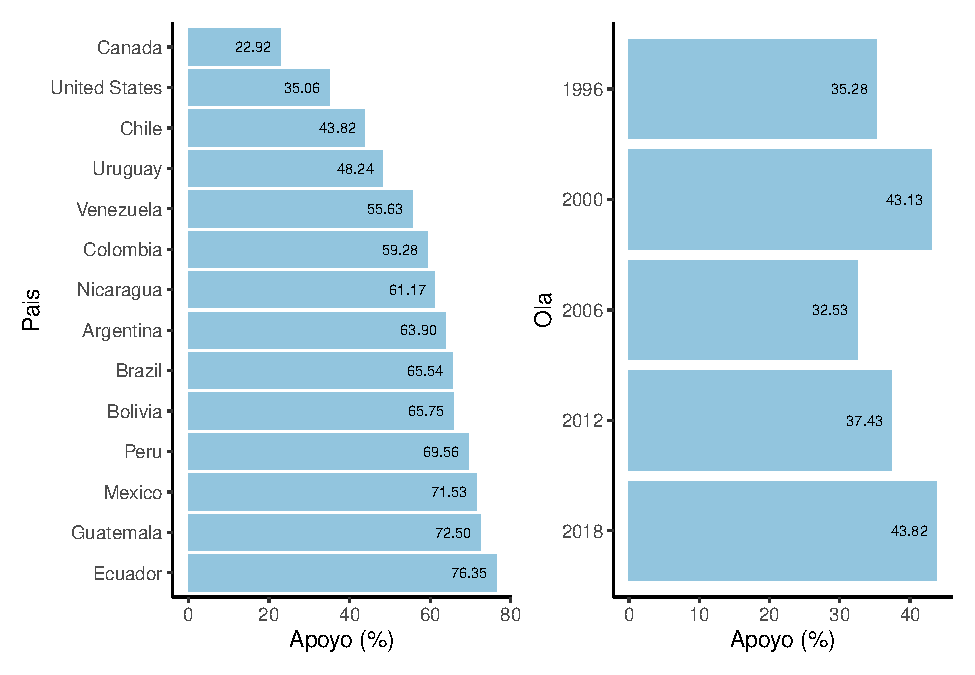
\includegraphics[width=1\linewidth,]{tesis_files/figure-latex/unnamed-chunk-5-1} \caption{Apoyo a Líder Fuerte en América (7ma Ola) y en Chile (1996-2018)}\label{fig:unnamed-chunk-5}
\end{figure}

\hypertarget{anuxe1lisis-de-clases-latentes-1}{%
\section{Análisis de Clases Latentes}\label{anuxe1lisis-de-clases-latentes-1}}

\hypertarget{anuxe1lisis-descriptivo-1}{%
\subsection*{Análisis Descriptivo}\label{anuxe1lisis-descriptivo-1}}
\addcontentsline{toc}{subsection}{Análisis Descriptivo}

\begin{figure}[!ht]

{\centering 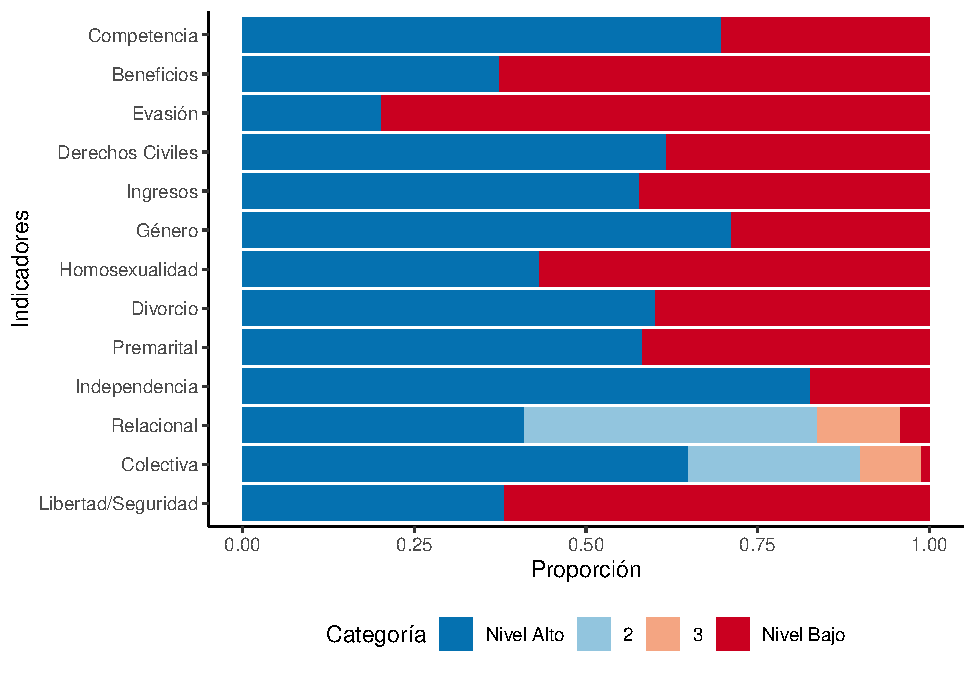
\includegraphics[width=0.5\linewidth,]{tesis_files/figure-latex/unnamed-chunk-6-1} 

}

\caption{Distribución indicadores de individualismo (recodificados)}\label{fig:unnamed-chunk-6}
\end{figure}
\FloatBarrier

Nota. Elaboración propia en base a datos de la Encuesta Mundial de Valores (Haerpfer et al., 2020); Todas las variables son dicotómicas, excepto los indicadores de independencia, interdependencia relacional e interdependencia colectiva, que no se recodificaron y se mantuvieron como variables categóricas de 4 categorías.

En la Figura 4.2 se presenta la distribución de los indicadores de individualismo para el total de la muestra. Se destaca una alta valoración de la competencia (70\%), pero un amplio rechazo al actuar estratégico cuando se trata de mentir para obtener beneficios sociales (63\%) o en la evasión en el transporte público (80\%). Además, se nota una valoración moderadamente alta de los indicadores de individualismo moral e individualismo expresivo.

El 83\% se siente a cargo de su vida, lo que refleja un alto nivel de independencia. De manera similar, un 84\% considera que hacer sentir orgullosos a sus padres es uno de los principales objetivos en sus vidas. Además, un 90\% de la población se siente cercana o muy cercana a su país. Estos hallazgos son coherentes con investigaciones previas que sugieren que las autoconcepciones independientes e interdependientes no son contradictorias, sino que muestran niveles igualmente altos en Chile \citep{benavides2020, kolstad2009}.

Por último, una proporción importante de la población (62\%) prioriza la seguridad (en rojo) por encima de la libertad (en azul). Este hallazgo -- que resulta interesante leerlo, además, a la luz de la crisis de seguridad que atraviesa el país actualmente -- podría representar evidencia a favor de que la autonomía no es el valor principal en base al cual las personas se constituyen como individuos en Chile \citep{martuccelli2010}.

\hypertarget{modelo-de-clases-latentes}{%
\subsection*{Modelo de Clases Latentes}\label{modelo-de-clases-latentes}}
\addcontentsline{toc}{subsection}{Modelo de Clases Latentes}

El siguiente paso, pues, es identificar si es posible identificar perfiles entre los que los indicadores seleccionados se comportan de manera diferenciada. Para llevar a cabo este análisis, se seleccionó un modelo de 4 clases en base a los estadísticos de ajuste, además de considerar criterios teóricos y de parsimonia \citep{collins2010}. El modelo seleccionado el cual se presenta a continuación en la Figura 4.4.

\begin{figure}[!ht]

{\centering 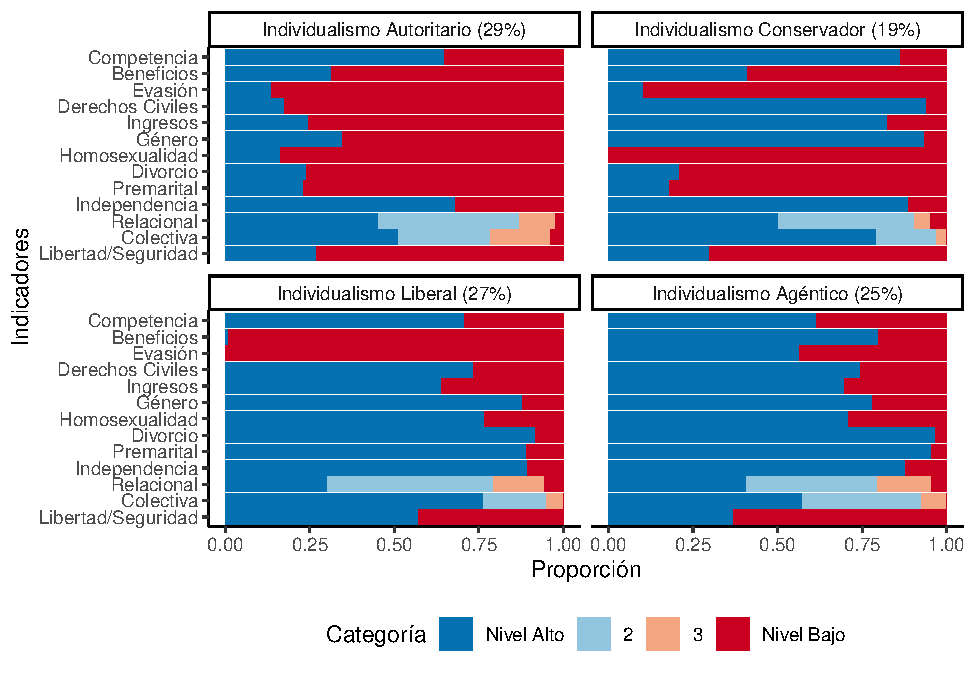
\includegraphics[width=1\linewidth,]{tesis_files/figure-latex/unnamed-chunk-7-1} 

}

\caption{Modelo de Clases Latentes de Individualismo (4 clases)}\label{fig:unnamed-chunk-7}
\end{figure}
\FloatBarrier

Nota. \(N\)=713; Parametros Estimados = 71; \(G^2\)= 3016,5 (df=642); \(AIC\)=11.812; \(BIC\)=12.136

Se observa que las cuatro clases muestran patrones distintos entre sí, así como diferencias respecto a la distribución promedio de la muestra. En la figura 4.5., se describe la distribución estimada de cada uno de los perfiles en la población.

\begin{figure}[!ht]

{\centering 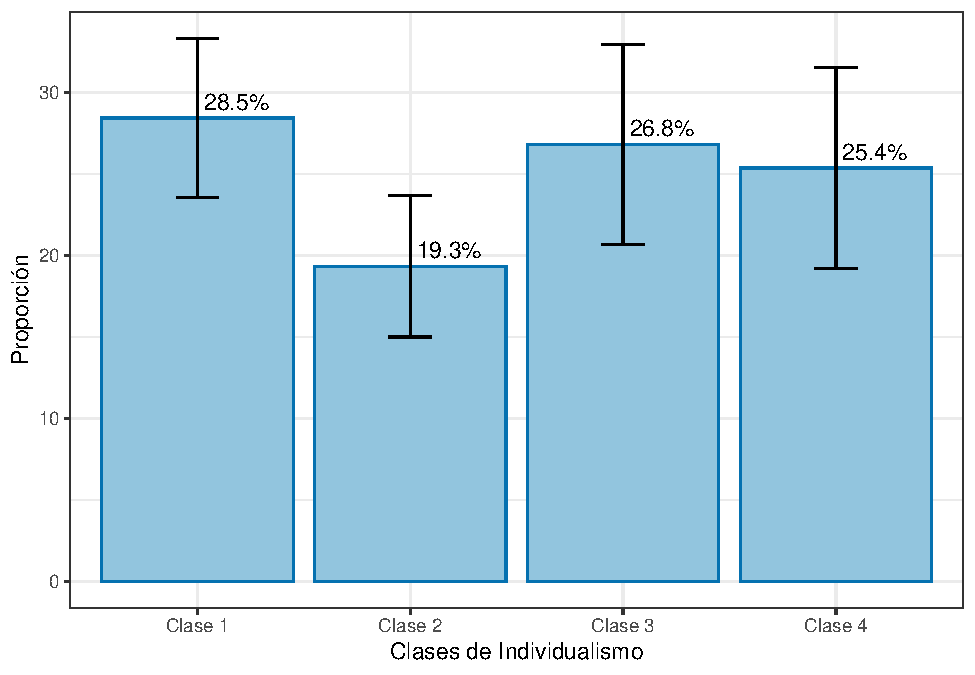
\includegraphics[width=1\linewidth,]{tesis_files/figure-latex/unnamed-chunk-8-1} 

}

\caption{Distribución estimada Clases Latentes}\label{fig:unnamed-chunk-8}
\end{figure}
\FloatBarrier

La clase 1 se caracteriza por valorar positivamente la competencia, pero a la vez tiende a rechazar la acción individual en diversas esferas. Por ejemplo, se observa un alto rechazo a evadir en el transporte público (88\%), una indiferencia hacia los derechos civiles (83\%), y un rechazo a la homosexualidad (84\%). Dicho en otras palabras, la acción individual cuenta con baja legitimidad tanto en la esfera económica, como en la política y en la expresiva. Para este grupo, de tal modo, la individualidad debe estar subsumida al respeto irrestricto a las normas sociales establecidas. Es posible que este deseo venga de una menor integración y de un mayor deseo por seguridad. Respecto a lo primero, es interesante destacar que esta clase presenta, además, el nivel más bajo de independencia (un igualmente alto 68\%) y de interdependencia colectiva (un 78\% se siente cercano o muy cercano al país). Asimismo, la probabilidad de que los miembros de esta clase prefieran la seguridad por sobre la libertad es la más alta entre las 4 clases, con un 73\%. Dado que la conformidad \citep{zakrisson2005} y la baja integración social \citep{gidron2020} son caracteristicas asociadas a las personalidades autoritarias, se ha decido bautizar a este perfil como \textbf{individualismo autoritario}

La edad promedio de este grupo es de 46,3 años, ligeramente superior al promedio de la muestra (44,3 años). Esta diferencia se debe principalmente a que solo el 14\% de las personas en este perfil tienen menos de 30 años {[}\^{}5{]}. Además, es importante señalar que este grupo muestra un mayor nivel de religiosidad, al menos en términos nominales: el 67\% de sus miembros se identifica como católico, mientras que solo el 19\% no tiene afiliación religiosa. Un rasgo adicional interesante de este perfil es que presenta, al mismo tiempo, la mayor proporción de personas pertenecientes a la clase trabajadora (48\%) y de personas de la clase de servicios (26\%).

La clase 2 se caracteriza por una alta probabilidad de justificar la competencia y de legitimar el individualismo moral, mientras que rechaza tanto la acción estratégica como la individualidad en la esfera expresiva. Esto se ve reflejado en las altas probabilidades, mayores a la del resto de los grupos, de rechazar la homosexualidad (100\%), el divorcio (79\%) y el sexo premarital (82\%). Por otro lado, parece ser el grupo donde la interdependencia relacional cobra más importancia en las autoconcepciones de los individuos. Por último, la probabilidad de que los miembros de esta clase prefieran la seguridad por encima de la libertad es del 70\%.

Al igual que el individualismo autoritario, este grupo se caracteriza por tener una edad promedio superior al de la muestra (47,8 años promedio). Esto se refleja en que la proporción de personas menores de 30 en este perfil alcanza solo el 12\%, mientras que el 28\% tiene 60 años o más. En general, los individualistas conservadores se encuentran políticamente más a la centro derecha (36\%), son más católicos (63\%) que otros grupos y viven en ciudades más pequeñas (el 27\% vive en ciudades menores a 100.000 habitantes). También es el grupo que más reporta ingresos subjetivos altos (14\%, el doble del promedio de la muestra). Sin embargo, esto no se ve reflejado en el tipo de trabajos que realizan, pues la proporción de personas pertenecientes a la clase media y clase de servicios en este perfil se encuentran en torno al promedio de la muestra.

El lema ``Dios, Patria y Familia'' podría describir bien a este grupo. ¿Qué lo diferencia del individualismo autoritario? Principalmente su mayor compromiso con los valores del individualismo moral. Por ejemplo, la probabilidad de presentar una alta valoración de los derechos civiles alcanza un 73\%. Por estos motivos, se ha decido denominar a este perfil como un \textbf{individualismo conservador}

La clase 3 tiene algunos rasgos similares con el individualismo conservador. Por ejemplo, muestra una alta probabilidad de legitimar la competencia, y también el individualismo moral, además de rechazar de forma considerable las acciones estratégicas. Sin embargo, se distancia de sus pares conservadores en dos aspectos fundamentales: Por un lado, en la alta legitimidad del individualismo expresivo que se observa en este grupo. Por otro, en que es la única clase donde la probabilidad de elegir la libertad es mayor que la de preferir la seguridad. Se le ha denomidado como \textbf{individualismo liberal}, pues, sus valores parecen apuntar al respeto a la libertad y a la tolerancia de la acción individual en todas las esferas de la vida social, aunque manteniendo el respeto por algunas normas de convivencia. A pesar de que podría asemejarse al ``individualismo institucional'' descrito por Martuccelli \citeyearpar{martuccelli2010}, se diferencia de este por su marcado carácter relacional -- lo que parece ser un rasgo transversal a las cuatro clases de individualismo identificadas.

Por un lado, este grupo se destaca por una mayor proporción de personas en la izquierda y la centro izquierda del espectro político (28\%), pero también el que alberga la mayor cantidad de personas sin identificación política (29\%). Por otro lado, en contraste con las dos clases anteriores, este grupo se muestra como menos religioso, con un 36\% de sus miembros declarando no tener afiliación religiosa. Es el perfil con la menor cantidad de personas pertenecientes a la clase trabajadora (40\%), pero presenta la mayor proporción de individuos pertenecientes a las clases intermedias (37\%).

Finalmente, la clase 4 se caracteriza por legitimar la acción individual en todas las esferas, incluyendo (y de manera única en este sentido) las acciones estratégicas. Aunque muestra niveles menores de interdependencia colectiva en comparación con sus pares liberales y conservadores, los niveles de independencia en esta clase son más altos que los observados en el individualismo autoritario. La preferencia por la seguridad por sobre la libertad en este grupo alcanza un 63\%, en torno al promedio de la población. Dado que es el único perfil que cuentan con una alta probabilidad de legitimar la acción individual en todas las esferas, se ha decidido denominar a este perfil como \textbf{individualismo estratégico}

De los cuatro perfiles, este es el único en el que se observan diferencias en la composición de género, mostrando una leve feminización (56\%). Además, es un grupo más joven, con una edad promedio de 40,3 años. El 28\% de las personas en esta clase son menores de 30 años, mientras que solo el 9\% tiene 60 años o más. A pesar de que el 64\% vive fuera de la Región Metropolitana, se diferencia del ``individualismo conservador'' en que se concentra en ciudades con más de 100,000 habitantes: es menos un individualismo de capitales provinciales y más un individualismo de capitales regionales. Comparte con el individualismo liberal una baja identificación religiosa, ya que el 37\% de sus miembros declara no tener religión. Finalmente, es el grupo que menos reporta ingresos subjetivos altos (4\%), el que más lo hace en ingresos subjetivos medios-bajos (57\%), y el que tiene la menor proporción de personas en las clases de servicios (20\%).

Para cerrar esta sección, y con el fin de ilustrar los principales hallazgos obtenidos a partir del análisis de clases latentes, la figura 4.6. presenta un resumen gráfico de las principales caracteristícas de los perfiles identificados.

\begin{figure}[!ht]

{\centering 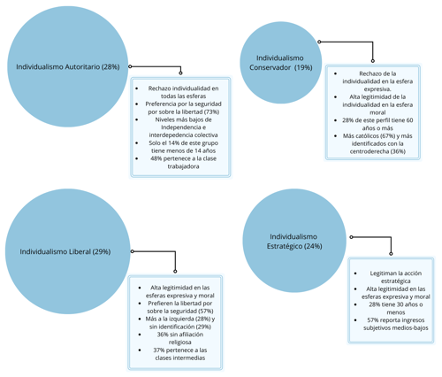
\includegraphics[width=1\linewidth,]{images/fig_esferas} 

}

\caption{Resumen Perfiles de Individualismo}\label{fig:nombre}
\end{figure}

\hypertarget{anuxe1lsis-de-varianza-y-modelos-de-regresiuxf3n}{%
\section{Análsis de Varianza y Modelos de Regresión}\label{anuxe1lsis-de-varianza-y-modelos-de-regresiuxf3n}}

En la tabla 4.1., se presenta el porcentaje de cada perfil de individualismo que valoraría como bueno o muy bueno a un liderazgo fuerte en el país. De tal modo, se puede observar que el Individualismo Estratégico y el Autoritario muestran los mayores niveles de apoyo, con un 53\% para ambos. Los niveles de apoyo en el Individualismo Conservador, en cambio, llegan a penas al 31\%, mientras que los del Individualismo Liberal se sitúan en torno al promedio (42\%). Mediante un Análisis de Varianza (ANOVA) es posible concluir que las diferencias entre los grupos son significativas (\(F\)= 6,47; \(p\)\textless0,001).

\begin{table}[h]

\caption{\label{tab:unnamed-chunk-9}Promedio Apoyo a Democracia Delegativa por perfiles de individualismo}
\begin{tabular}[t]{>{\centering\arraybackslash}m{5.2cm}>{\centering\arraybackslash}m{2.8cm}>{}m{2.8cm}>{}m{2.8cm}}
\toprule
Perfiles & Apoyo a Lideres Fuertes\\
\midrule
Individidualismo Autoritario & 52,51\\
Individualismo Conservador & 30,71\\
Individualismo Liberal & 41,71\\
Individualismo Estratégico & 52,60\\
\bottomrule
\end{tabular}
\end{table}
\FloatBarrier

En la tabla X, se presentan los modelos estimados para predicir el apoyo a un líder fuerte en Chile. En el Modelo 1, se incluye como único predictor el individualismo, que se ha convertido en una variable categórica a partir de las probabilidades posteriores estimadas por el modelo de clases latentes. Se especificó al Individualismo Conservador como variable de referencia, ya que esto permitiría apreciar mejor las diferencias entre los grupos. De tal modo, en relación a ser un individualista conservador, ser un individualista autoritario (\(OR\)=2,5; \(p\)\textless0,05), un individualista estratégico (\(OR\)=2,5; \(p\)\textless0,001) o un individualista liberal (\(OR\)=1,6; \(p\)\textless0,001) estaría asociado a un efecto positivo y significativo en el apoyo a un líder fuerte. Ahora bien, una vez que se agregan las variables de control al modelo, la asociación del individualismo liberal con el apoyo a un líder fuerte deja de ser significativa (\(OR\)=1,6; \(p\)\textless0,12). En cambio, las asociaciones con el individualismo autoritario (\(OR\)=3,1; \(p\)\textless0,001) y el individualismo estratégico (\(OR\)=2,9; \(p\)\textless0,001) se mantienen positivas y significativas.

\begin{verbatim}
## Warning: fonts used in `flextable` are ignored because the `pdflatex` engine is
## used and not `xelatex` or `lualatex`. You can avoid this warning by using the
## `set_flextable_defaults(fonts_ignore=TRUE)` command or use a compatible engine
## by defining `latex_engine: xelatex` in the YAML header of the R Markdown
## document.
\end{verbatim}

\global\setlength{\Oldarrayrulewidth}{\arrayrulewidth}

\global\setlength{\Oldtabcolsep}{\tabcolsep}

\setlength{\tabcolsep}{0pt}

\renewcommand*{\arraystretch}{1.5}



\providecommand{\ascline}[3]{\noalign{\global\arrayrulewidth #1}\arrayrulecolor[HTML]{#2}\cline{#3}}

\begin{longtable}[c]{ccc}

\caption{Modelos\ de\ Regresión\ Logística\ (Estimación\ de\ Odds\ Ratio)}\label{tab:unnamed-chunk-10}\\

\ascline{1.5pt}{666666}{1-3}

\multicolumn{1}{>{}c}{\textcolor[HTML]{000000}{\fontsize{11}{11}\selectfont{\ }}} & \multicolumn{1}{>{}c}{\textcolor[HTML]{000000}{\fontsize{11}{11}\selectfont{(1)}}} & \multicolumn{1}{>{}c}{\textcolor[HTML]{000000}{\fontsize{11}{11}\selectfont{(3)}}} \\

\ascline{1.5pt}{666666}{1-3}\endfirsthead \caption[]{Modelos\ de\ Regresión\ Logística\ (Estimación\ de\ Odds\ Ratio)}\label{tab:unnamed-chunk-10}\\

\ascline{1.5pt}{666666}{1-3}

\multicolumn{1}{>{}c}{\textcolor[HTML]{000000}{\fontsize{11}{11}\selectfont{\ }}} & \multicolumn{1}{>{}c}{\textcolor[HTML]{000000}{\fontsize{11}{11}\selectfont{(1)}}} & \multicolumn{1}{>{}c}{\textcolor[HTML]{000000}{\fontsize{11}{11}\selectfont{(3)}}} \\

\ascline{1.5pt}{666666}{1-3}\endhead



\multicolumn{3}{>{}c}{\textcolor[HTML]{000000}{\fontsize{11}{11}\selectfont{Nota.\ *:p<0,05;\ **:p<0.01;\ ***p<0.001}}} \\

\endfoot



\multicolumn{1}{>{}c}{\textcolor[HTML]{000000}{\fontsize{11}{11}\selectfont{Constante}}} & \multicolumn{1}{>{}c}{\textcolor[HTML]{000000}{\fontsize{11}{11}\selectfont{0.443***}}} & \multicolumn{1}{>{}c}{\textcolor[HTML]{000000}{\fontsize{11}{11}\selectfont{0.169**}}} \\





\multicolumn{1}{>{}c}{\textcolor[HTML]{000000}{\fontsize{11}{11}\selectfont{Autoritario}}} & \multicolumn{1}{>{}c}{\textcolor[HTML]{000000}{\fontsize{11}{11}\selectfont{2.495***}}} & \multicolumn{1}{>{}c}{\textcolor[HTML]{000000}{\fontsize{11}{11}\selectfont{3.161***}}} \\





\multicolumn{1}{>{}c}{\textcolor[HTML]{000000}{\fontsize{11}{11}\selectfont{Liberal}}} & \multicolumn{1}{>{}c}{\textcolor[HTML]{000000}{\fontsize{11}{11}\selectfont{1.615*}}} & \multicolumn{1}{>{}c}{\textcolor[HTML]{000000}{\fontsize{11}{11}\selectfont{1.564}}} \\





\multicolumn{1}{>{}c}{\textcolor[HTML]{000000}{\fontsize{11}{11}\selectfont{Estratégico}}} & \multicolumn{1}{>{}c}{\textcolor[HTML]{000000}{\fontsize{11}{11}\selectfont{2.504***}}} & \multicolumn{1}{>{}c}{\textcolor[HTML]{000000}{\fontsize{11}{11}\selectfont{2.853***}}} \\





\multicolumn{1}{>{}c}{\textcolor[HTML]{000000}{\fontsize{11}{11}\selectfont{Mujer}}} & \multicolumn{1}{>{}c}{\textcolor[HTML]{000000}{\fontsize{11}{11}\selectfont{}}} & \multicolumn{1}{>{}c}{\textcolor[HTML]{000000}{\fontsize{11}{11}\selectfont{1.437}}} \\





\multicolumn{1}{>{}c}{\textcolor[HTML]{000000}{\fontsize{11}{11}\selectfont{Edad}}} & \multicolumn{1}{>{}c}{\textcolor[HTML]{000000}{\fontsize{11}{11}\selectfont{}}} & \multicolumn{1}{>{}c}{\textcolor[HTML]{000000}{\fontsize{11}{11}\selectfont{0.991}}} \\





\multicolumn{1}{>{}c}{\textcolor[HTML]{000000}{\fontsize{11}{11}\selectfont{Izquierda}}} & \multicolumn{1}{>{}c}{\textcolor[HTML]{000000}{\fontsize{11}{11}\selectfont{}}} & \multicolumn{1}{>{}c}{\textcolor[HTML]{000000}{\fontsize{11}{11}\selectfont{1.265}}} \\





\multicolumn{1}{>{}c}{\textcolor[HTML]{000000}{\fontsize{11}{11}\selectfont{Centro\ Izquierda}}} & \multicolumn{1}{>{}c}{\textcolor[HTML]{000000}{\fontsize{11}{11}\selectfont{}}} & \multicolumn{1}{>{}c}{\textcolor[HTML]{000000}{\fontsize{11}{11}\selectfont{1.094}}} \\





\multicolumn{1}{>{}c}{\textcolor[HTML]{000000}{\fontsize{11}{11}\selectfont{Centro}}} & \multicolumn{1}{>{}c}{\textcolor[HTML]{000000}{\fontsize{11}{11}\selectfont{}}} & \multicolumn{1}{>{}c}{\textcolor[HTML]{000000}{\fontsize{11}{11}\selectfont{1.245}}} \\





\multicolumn{1}{>{}c}{\textcolor[HTML]{000000}{\fontsize{11}{11}\selectfont{Centro\ Derecha}}} & \multicolumn{1}{>{}c}{\textcolor[HTML]{000000}{\fontsize{11}{11}\selectfont{}}} & \multicolumn{1}{>{}c}{\textcolor[HTML]{000000}{\fontsize{11}{11}\selectfont{0.754}}} \\





\multicolumn{1}{>{}c}{\textcolor[HTML]{000000}{\fontsize{11}{11}\selectfont{Derecha}}} & \multicolumn{1}{>{}c}{\textcolor[HTML]{000000}{\fontsize{11}{11}\selectfont{}}} & \multicolumn{1}{>{}c}{\textcolor[HTML]{000000}{\fontsize{11}{11}\selectfont{2.890}}} \\





\multicolumn{1}{>{}c}{\textcolor[HTML]{000000}{\fontsize{11}{11}\selectfont{Ingresos\ Subjetivos}}} & \multicolumn{1}{>{}c}{\textcolor[HTML]{000000}{\fontsize{11}{11}\selectfont{}}} & \multicolumn{1}{>{}c}{\textcolor[HTML]{000000}{\fontsize{11}{11}\selectfont{1.086}}} \\





\multicolumn{1}{>{}c}{\textcolor[HTML]{000000}{\fontsize{11}{11}\selectfont{Católica}}} & \multicolumn{1}{>{}c}{\textcolor[HTML]{000000}{\fontsize{11}{11}\selectfont{}}} & \multicolumn{1}{>{}c}{\textcolor[HTML]{000000}{\fontsize{11}{11}\selectfont{1.693*}}} \\





\multicolumn{1}{>{}c}{\textcolor[HTML]{000000}{\fontsize{11}{11}\selectfont{Evangélica}}} & \multicolumn{1}{>{}c}{\textcolor[HTML]{000000}{\fontsize{11}{11}\selectfont{}}} & \multicolumn{1}{>{}c}{\textcolor[HTML]{000000}{\fontsize{11}{11}\selectfont{1.635}}} \\





\multicolumn{1}{>{}c}{\textcolor[HTML]{000000}{\fontsize{11}{11}\selectfont{Otra}}} & \multicolumn{1}{>{}c}{\textcolor[HTML]{000000}{\fontsize{11}{11}\selectfont{}}} & \multicolumn{1}{>{}c}{\textcolor[HTML]{000000}{\fontsize{11}{11}\selectfont{1.359}}} \\





\multicolumn{1}{>{}c}{\textcolor[HTML]{000000}{\fontsize{11}{11}\selectfont{Rural}}} & \multicolumn{1}{>{}c}{\textcolor[HTML]{000000}{\fontsize{11}{11}\selectfont{}}} & \multicolumn{1}{>{}c}{\textcolor[HTML]{000000}{\fontsize{11}{11}\selectfont{0.624}}} \\





\multicolumn{1}{>{}c}{\textcolor[HTML]{000000}{\fontsize{11}{11}\selectfont{Menos\ de\ 100.000hab}}} & \multicolumn{1}{>{}c}{\textcolor[HTML]{000000}{\fontsize{11}{11}\selectfont{}}} & \multicolumn{1}{>{}c}{\textcolor[HTML]{000000}{\fontsize{11}{11}\selectfont{0.557*}}} \\





\multicolumn{1}{>{}c}{\textcolor[HTML]{000000}{\fontsize{11}{11}\selectfont{Más\ de\ 100.000hab}}} & \multicolumn{1}{>{}c}{\textcolor[HTML]{000000}{\fontsize{11}{11}\selectfont{}}} & \multicolumn{1}{>{}c}{\textcolor[HTML]{000000}{\fontsize{11}{11}\selectfont{1.675*}}} \\





\multicolumn{1}{>{}c}{\textcolor[HTML]{000000}{\fontsize{11}{11}\selectfont{Clase\ Media}}} & \multicolumn{1}{>{}c}{\textcolor[HTML]{000000}{\fontsize{11}{11}\selectfont{}}} & \multicolumn{1}{>{}c}{\textcolor[HTML]{000000}{\fontsize{11}{11}\selectfont{1.308}}} \\





\multicolumn{1}{>{}c}{\textcolor[HTML]{000000}{\fontsize{11}{11}\selectfont{Clase\ Trabajadora}}} & \multicolumn{1}{>{}c}{\textcolor[HTML]{000000}{\fontsize{11}{11}\selectfont{}}} & \multicolumn{1}{>{}c}{\textcolor[HTML]{000000}{\fontsize{11}{11}\selectfont{1.423}}} \\

\ascline{1pt}{000000}{1-3}



\multicolumn{1}{>{}c}{\textcolor[HTML]{000000}{\fontsize{11}{11}\selectfont{\$N\$}}} & \multicolumn{1}{>{}c}{\textcolor[HTML]{000000}{\fontsize{11}{11}\selectfont{647}}} & \multicolumn{1}{>{}c}{\textcolor[HTML]{000000}{\fontsize{11}{11}\selectfont{550}}} \\

\ascline{1.5pt}{666666}{1-3}



\end{longtable}



\arrayrulecolor[HTML]{000000}

\global\setlength{\arrayrulewidth}{\Oldarrayrulewidth}

\global\setlength{\tabcolsep}{\Oldtabcolsep}

\renewcommand*{\arraystretch}{1}

\FloatBarrier

Para empezar a comprender las consecuencias que estas asociaciones pueden tener para la democracia en Chile, se presenta en la figura X un análisis que permite observar las diferencias en participación política entre las clases de individualismo identificados. Se debe recordar que, hasta 2022, el voto en Chile era voluntario y que la participación electoral en las elecciones presidenciales del año 2017 (última previa a la encuesta) fue de 47\% en primera vuelta y del 49\% en el balotaje.

De tal modo, los datos apuntan a que los perfiles de individualismo que en 2018 participaban menos de las elecciones presidenciales se corresponden justamente con aquellos que tienden a mostrar un apoyo a un líder fuerte. Así, mientras la proporción de individualistas liberales y conservadores que votan siempre en las elecciones presidenciales se eleva hasta el 60\%. En cambio, entre individualistas estratégicos y autoritarios esa cifra no llega al 40\%. Esto es consistente con otros trabajos que han apuntado a que los nuevos votantes chilenos muestran mayores tendencias autoritarias que los votantes habituales \citep{coes2023}.

\begin{figure}[!ht]

{\centering 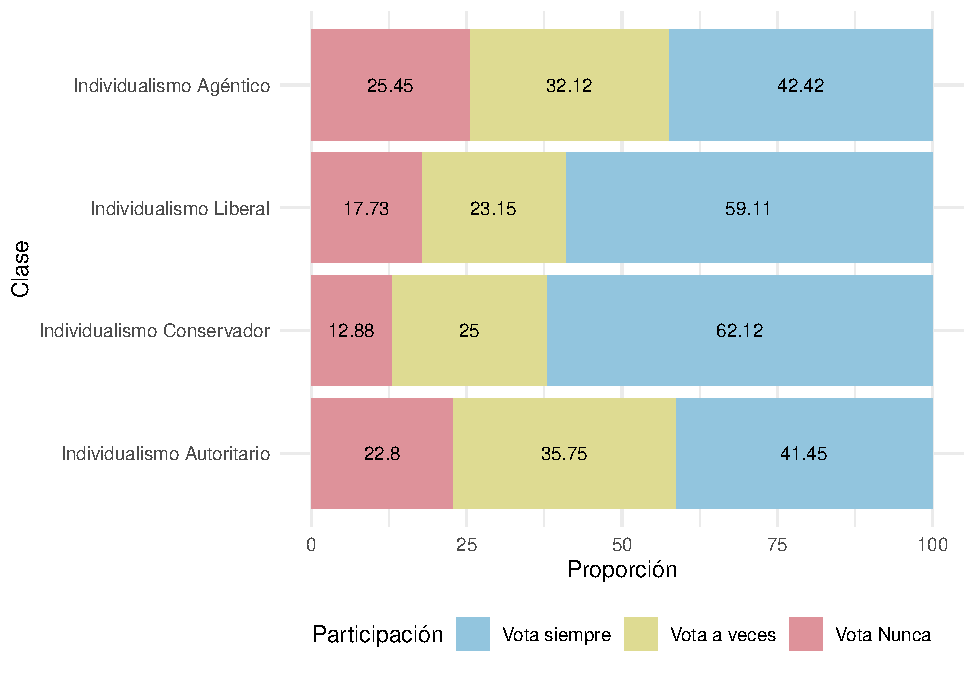
\includegraphics[width=1\linewidth,]{tesis_files/figure-latex/unnamed-chunk-11-1} 

}

\caption{Perfiles de Individualismo por participación política}\label{fig:unnamed-chunk-11}
\end{figure}

\hypertarget{discusiuxf3n}{%
\chapter{Discusión}\label{discusiuxf3n}}

\textbf{Apoyo a la Líderes Fuertes}

Según datos de la Encuesta Mundial de Valores, el 44\% de la población chilena consideraría como bueno o muy buena contar con un líder fuerte que no le importen el congreso o las elecciones. Si bien esta cifra puede considerarse como baja en el contexto latinoamericano, donde los niveles de apoyo a un líder fuerte se encuentran sobre el 50\% en prácticamente todos los países de la región sondeados, se debe destacar una tendencia al alza sostenida entre el 2006 y el 2018, creciendo 12 puntos porcentuales en ese período.

Los datos que pueda entregar la Octava Ola de la Encuesta Mundial de Valores, que debieran estar disponibles a más tardar en 2026, van a ser interesantes para constatar si esta tendencia ha continuado durante el último lustro. Al respecto, es importantes destacar que los datos disponibles son anteriores a fenómenos sociales de gran importancia que podrían influir en como los ciudadanos evalúan este tipo de líderes, como el Estallido Social del 2019, la pandemia por COVID-19, la crisis migratoria y de seguridad, así como la irrupción de liderazgos autoritarios tanto en el contexto nacional como latinoamericano.

\textbf{Perfiles de Individualismo}

El análisis de clases latentes realizado respalda la hipótesis de que los procesos de individualización divergen dentro de una misma sociedad. A partir de los datos examinados, se logró identificar cuatro perfiles distintos de individualismo en la sociedad chilena: individualismo autoritario, individualismo conservador, individualismo liberal e individualismo agéntico. Cada uno de estos perfiles equivale a variadas representaciones de la posición del individuo en la sociedad, y son resultado de combinaciones específicas de legitimidad de la acción individual en diferentes esferas, concepciones variadas del individuo, y diferentes valores e imperativos estructuralmente producidos. Además, la presencia de diferencias en edad, orientación política, ubicación geográfica o afiliación religiosa entre estos perfiles arroja luz sobre cómo los procesos estructurales interactúan de manera diferenciada con distintos segmentos de la población.

La tipología elaborada permite establecer un diálogo con la descripción del individualismo agéntico y el híper-actor relacional propuesto por Araujo y Martuccelli \citeyearpar{araujo2020}. Este modelo presenta dos características fundamentales: en primer lugar, la confianza depositada en las habilidades personales para afrontar la vida social, y en segundo lugar, la centralidad de las redes interpersonales. Se observó que una de las clases identificadas se acerca de manera más nítida a este modelo, de ahí que se haya decidido mantener la denominación de ``individualismo agéntico''. No obstante, se debe destacar que los otros perfiles también exhiben rasgos que hacen suponer que comparten, al menos parcialmente, la descripción de Araujo y Martuccelli.

En relación con la confianza en el esfuerzo y las habilidades personales, esto podría observarse en la alta valoración de la competencia y los elevados niveles de independencia observados de manera transversal en todos los perfiles. En términos generales, los datos sugieren que la mayoría de los chilenos cree poseer las habilidades necesarias para asumir el control de sus propias vidas.

Por otro lado, el carácter relacional del individualismo chileno parece ser una característica que atraviesa todos los perfiles \citep{araujo2014}. Cierto es que se mide solo una identidad relacional (la familiar) y solo una identidad colectiva (la nacional). Pese a esto, no parece demasiado difícil argumentar la importancia de estas identidades y que incluirlas en el modelo sirve para un buen primer acercamiento.

También es importante señalar que el carácter relacional del individualismo chileno parece no entrar en contradicción con las concepciones independientes, que muestran niveles tan elevados como los indicadores de interdependencia. Esto es consistente tanto con las dos características que describen al individualismo agéntico \citep{araujo2020} como con las investigaciones sobre el \emph{self-construal} en Chile \citep{benavides2020, kolstad2009}. Además, ofrece más respaldo a la idea de que ubicar a Chile en un continuo entre el individualismo y el colectivismo resulta problemático.

En resumen, a partir de los datos analizados, se puede concluir que el individualismo agéntico representa el modelo predominante de individualismo en Chile. Sin embargo, el aporte de esta investigación radica en que, mediante el análisis de clases latentes, es posible observar cómo este modelo diverge dentro de la sociedad chilena. Para algunos, la acción individual debe estar subordinada al orden normativo, mientras que para otros es legítimo actuar de manera estratégica incluso si ello transgrede normas sociales. Mientras que para unos la individualidad tiene cabida en todas las esferas, para otros su legitimidad no alcanza para la esfera afectiva. De tal modo, este enfoque permite observar los matices y las divergencias de los procesos de individualización en Chile.

\textbf{Apoyo a la democracia delegativa y perfiles de individualismo}

El hecho de que haya sido posible establecer una relación estadísticamente significativa entre los perfiles de individualismo y el respaldo a liderazgos fuertes debe ser considerado como una evidencia alentadora del potencial del modelo teórico de individualismo propuesto. Dos de los perfiles identificados muestran una asociación negativa con el apoyar a este tipo de líderes (el conservador y el liberal), mientras que los otros dos (el agéntico y el autoritario) presentan una relación positiva. También es importante destacar que en aquellos que muestran mayores niveles de apoyo son justamente quienes presentaban una menor participación electoral en 2018, en un contexto de voto voluntario.

Cabe preguntarse si este no es un eje que permita distinguir entre los perfiles identificados: el individualismo conservador y el liberal podrían denominarse como \emph{individualismos cívicos}, orientados hacia lo público. En contraste, el autoritario y el agéntico podrían considerarse más bien \emph{hiperindividualismos}, que están orientados más bien hacia lo privado. En los primeros, la individualidad estaría vinculada a la pertenencia a una comunidad política; en los segundos, lo público representaría un desafío, un obstáculo que se debe evitar ya sea mediante la sumisión de la individualidad a un orden normativo (como en el caso del individualismo autoritario) o mediante la maximización de las habilidades personales (como es el caso del individualismo estratégico).

Tomando en consideración las diferencias en participación política entre los perfiles, cabe reflexionar sobre las consecuencias de estos hallazgos sobre la democracia chileno, particularmente considerando que ahora los grupos que muestran un mayor apoyo a los líderes fuertes están obligados a votar, en un contexto de crisis de seguridad y en que el denominado ``estilo Bukele'' empieza a ganar adherentes en el país.
Si bien otros estudios \citep{coes2023} han notado la mayor tendencia hacia el autoritarismo y el conservadurismo de los nuevos votantes, cabe preguntarse si es el único fenómeno aquí presente. Normalmente, se ha considerado que la submisión de la autonomía a la autoridad es un rasgo propio de las personalidades autoridades. Si bien esto se observaría en el individualismo autoritario, no es el caso el individualismo estratégico ¿Porque un grupo de la población que valor y legitima la acción individual en todas las esferas estaría predipuesto a liderazgos dominantes?

Una respuesta se puede encontrar en, como se menciona en la Encuesta Nacional de la Autoridad \citep{araujo2022}, la autoridad política estaría sostenida en la eficacia de los liderazgos para cumplir sus tareas. Esto en un contexto que Juan Pablo Luna \citeyearpar{luna2016} ha denominado como ``Democracia Desarraigada'', donde existe una fuerte desconexión entre ciudadanos y élite política. De tal modo, sería posible hipotetizar que el deseo de los chilenos -- particularmente de los \emph{hiperindividualistas} -- por liderazgos fuertes no es puro autoritarismo, sino la demanda por un tipo de autoridad que se podría denominar como \emph{delegativa} \citep{odonnell1994}. En una democracia delegativa, los ciudadanos podrían ejercer el voto periódicamente para luego retirarse de la esfera pública hasta la próxima elección \citep{peruzzotti2008}. Pero esta apatía está lejos de ser un cheque en blanco: al líder electo se le exigen resultados, incluso si ello implica transgredir la autonomía de otras instituciones del Estado. Los hiperindividualistas, así, no estarían -- necesariamente -- en contra de la democracia, pero sí tendrían una visión más pragmática de esta.

En resumen, esta investigación sugiere que la relación entre el individualismo y el apoyo a lideres fuertes es significativa, pero divergente entre distintos grupos. En otras palabras, distintas formas de individualismos, resultado de divergencias en los procesos de individuación, preferían formas distintas de ejercer la autoridad. Mientras que los individualismos cívicos parecen valorar una visión más representativa de la democracia, los hiperindividualismos favorecen un enfoque más pragmático y apático hacia la esfera pública. Esto ilustra un panorama general en el que las manifestaciones del individualismo, y su relación con otros fenómenos, aparecen como más complejas de lo que otros estudios han propuesto.

\hypertarget{conclusiuxf3n}{%
\chapter{Conclusión}\label{conclusiuxf3n}}

Para cerrar, se presentarán algunas reflexiones sobre las limitaciones y posibles líneas de investigación futuras que se desprenden de este estudio.

Es importante reflexionar sobre las oportunidades que brinda el análisis de clases latentes en la investigación sobre los procesos de individualización en Chile. Dada la dificultad para traducir su marco teórico a una propuesta metodológica mediante las técnicas cuantitativas más comunes, la sociología del individuo se ha desarrollado principalmente desde una perspectiva cualitativa, resultando en descripciones profundas y estimulantes sobre el individuo en la sociedad chilena. Pese a ello, el enfoque metodológico adoptado en esta investigación permitió identificar algunos de los rasgos del individualismo agéntico descritos por Araujo y Martuccelli \citeyearpar{araujo2014}, al tiempo que ofrece una visión más matizada de cómo los procesos de individuación divergen en la sociedad chilena, diferenciándose entre grupos sociales y teniendo consecuencias en las actitudes políticas de los individuos.

Por supuesto, enfoques cualitativos y cuantitativos no deben ser vistos como competitivos, sino como complementarios en el desarrollo de una sociología del individuo. Las propias conclusiones aquí delineadas, y las hipótesis que de ellas se desprenden, se verían fuertemente enriquecidas si se incluyeran datos cualitativos que permitirían obtener una compresión más profunda de las distintas variantes de individualismo y su relación divergente con la esfera pública.

Ahora bien, es necesario reconocer las limitaciones que enfrentó esta investigación. La principal, posiblemente, se derive de los indicadores seleccionados. Aunque los resultados obtenidos parecen prometedores, es crucial continuar avanzando en la construcción y validación de indicadores que permitan traducir el modelo teórico aquí propuesto en un modelo de medición capaz de abordar el fenómeno del individualismo en Chile. En particular, las operacionalizaciones del individualismo utilitario, del individualismo moral, de la interdependencia relacional y de la interdependencia colectiva merecen, sin duda, un mayor trabajo metodológico y conceptual que permitan construir y validar indicadores en esas dimensiones.

Por otro lado , la recodificación de variables continuas como dicotómicas es una solución pragmática, pero que no deja de ser problemática, ya que resulta en la pérdida de parte de la varianza de los ítems \citep{fernandes2019}. Futuras investigaciones deberían considerar elaborar indicadores directamente como variables categóricas que no necesiten recodificación para ser incluidas en el modelo de clases latentes. De esta manera, se obtendría claridad en los resultados sin sacrificar información ni poder estadístico.

Otras limitaciones provienen más bien de la muestra. Si 5 años ya se encuentra en el límite de lo que se puede considerar como datos relevantes para la actualidad, a esto se debe sumar que este último lustro ha sido uno particularmente tumultuoso: el Estallido Social, la Pandemia, el proceso constituyente, la crisis migratoria y la crisis de seguridad han sido algunos de los eventos de gran magnitud que han marcado la agenda durante los últimos años. ¿Están hoy los chilenos más dispuestos que hace 5 años a sacrificar su libertad y su individualidad en distintas esferas para obtener garantías de orden y seguridad? Entre las ollas comunes y los retiros de fondos previsionales, entre las protestas masivas y las cuarentenas, ¿cambiaron las concepciones -- independientes, relacionales y colectivas -- con las que los individuos construyen sus identidades? ¿Qué efectos puede tener la instauración del voto obligatorio en el eje individualismo cívico-hiperindividualismo, o en las percepciones de los ciudadanos sobre las formas en que se ejercer la autoridad? Todas estas son preguntas relevantes que quedarán abiertas y deberán ser abordadas en el futuro.

A su vez, dado que Chile ha participado en 6 olas de la Encuesta Mundial de Valores desde 1990, se debería considerar correr los modelos aquí propuestos utilizando datos de ediciones anteriores (así como estar atento a la próxima versión a realizarse entre 2023 y 2026). Esto permitiría evaluar si los resultados obtenidos en este estudio guardan consistencia con el pasado, así como observar la evolución de estos indicadores a lo largo del tiempo.

Pese a estas limitaciones, el trabajo contenido en este documento logra obtener resultados relevantes. Se encontró evidencia de que distintas formas de individualismo pueden generar actitudes políticas diferentes respecto a los tipos de liderazgos esperados por la ciudadanía. Es importante considerar que estas inclinaciones no surgen en un vacío, sino que son el resultado de la interacción de factores institucionales y estructurales con la agencia de los individuos. De esta manera, se espera que la lectura de esta investigación provoque la reflexión en torno a los tipos de individuos que nuestras instituciones, a través de sus programas e incentivos, contribuyen a producir, así como en las consecuencias de estos procesos para la democracia chilena y la vida social en general.

% %%%%%%%%%%%%%%%%%%%%%%%%%%%%%%%%%%%%%%%%%%%%%%%%%
% %%% Bibliography                              %%%
% %%%%%%%%%%%%%%%%%%%%%%%%%%%%%%%%%%%%%%%%%%%%%%%%%
%\addtocontents{toc}{\vspace{.9\baselineskip}}

\pagestyle{fancyplain}
\fancyhf{}
	 \fancyhead[RE]{\slshape Bibliografía}
	 \fancyfoot[C]{\thepage}
\phantomsection
\addcontentsline{toc}{chapter}{Bibliografía}
\bibliography{tesis}

%% All books from our library (SfS) are already in a BiBTeX file
%% (Assbib). You can use Assbib combined with your personal BiBTeX file:
%% \bibliography{Myreferences,Assbib}. Of course, this will only work on
%% the computers at SfS, unless you copy the Assbib file
%%  --> /u/sfs/bib/Assbib.bib


\hypertarget{Anexo}{%
\chapter*{Anexo}\label{Anexo}}
\addcontentsline{toc}{chapter}{Anexo}

\begin{table}[!h]

\caption{\label{tab:unnamed-chunk-14}Indicadores Sociodemográficos por Perfiles de Individualismo}
\fontsize{8}{10}\selectfont
\begin{tabu} to \linewidth {>{\raggedright}X>{\raggedleft}X>{\raggedleft}X>{\raggedleft}X>{\raggedleft}X}
\toprule
\multicolumn{1}{c}{Indicador} & \multicolumn{1}{c}{Autoritario} & \multicolumn{1}{c}{Conservador} & \multicolumn{1}{c}{Liberal} & \multicolumn{1}{c}{Agéntico}\\
\midrule
\addlinespace[0.3em]
\multicolumn{5}{l}{\textbf{Edad}}\\
\hspace{1em}30 a 44 & 34,00 & 34,59 & 36,27 & 33,73\\
\hspace{1em}45 a 59 & 30,00 & 27,07 & 28,43 & 28,99\\
\hspace{1em}Mayores de 60 & 21,50 & 26,32 & 15,69 & 9,47\\
\hspace{1em}Menores de 30 & 14,50 & 12,03 & 19,61 & 27,81\\
\addlinespace[0.3em]
\multicolumn{5}{l}{\textbf{Género}}\\
\hspace{1em}Hombre & 51,50 & 48,87 & 50,49 & 44,97\\
\hspace{1em}Mujer & 48,50 & 51,13 & 49,51 & 55,03\\
\addlinespace[0.3em]
\multicolumn{5}{l}{\textbf{Identificación Política}}\\
\hspace{1em}Ninguna & 24,00 & 16,54 & 28,92 & 23,08\\
\hspace{1em}Izquierda & 4,50 & 0,00 & 8,33 & 7,10\\
\hspace{1em}Centro Izquierda & 21,00 & 23,31 & 19,61 & 24,26\\
\hspace{1em}Centro & 28,00 & 24,81 & 23,53 & 21,30\\
\hspace{1em}Centro Derecha & 21,00 & 35,34 & 15,20 & 21,30\\
\hspace{1em}Derecha & 1,50 & 0,00 & 4,41 & 2,96\\
\addlinespace[0.3em]
\multicolumn{5}{l}{\textbf{Ingresos Subjetivos}}\\
\hspace{1em}Ingresos Altos & 7,00 & 13,53 & 4,41 & 4,14\\
\hspace{1em}Ingresos Bajos & 19,50 & 15,79 & 17,65 & 13,61\\
\hspace{1em}Ingresos Medios-Altos & 28,50 & 18,05 & 26,47 & 24,85\\
\hspace{1em}Ingresos Medios-Bajos & 45,00 & 52,63 & 51,47 & 57,40\\
\addlinespace[0.3em]
\multicolumn{5}{l}{\textbf{Religion}}\\
\hspace{1em}Sin religión & 19,07 & 21,21 & 35,18 & 36,42\\
\hspace{1em}Católica & 67,01 & 62,88 & 55,28 & 53,70\\
\hspace{1em}Evangélica & 7,22 & 8,33 & 6,03 & 4,94\\
\hspace{1em}Otra & 6,70 & 7,58 & 3,52 & 4,94\\
\addlinespace[0.3em]
\multicolumn{5}{l}{\textbf{Tipo de Ciudad}}\\
\hspace{1em}Santiago & 44,00 & 28,57 & 38,73 & 36,09\\
\hspace{1em}Rural & 13,50 & 9,77 & 13,24 & 13,02\\
\hspace{1em}Menos de 100.000 & 17,00 & 26,32 & 11,76 & 14,20\\
\hspace{1em}Sobre 100.000 & 25,50 & 35,34 & 36,27 & 36,69\\
\addlinespace[0.3em]
\multicolumn{5}{l}{\textbf{Clase Social}}\\
\hspace{1em}Clase de Servicio & 26,16 & 23,93 & 23,30 & 20,67\\
\hspace{1em}Clase Media & 26,16 & 34,19 & 36,93 & 37,33\\
\hspace{1em}Clase Trabajadora & 47,67 & 41,88 & 39,77 & 42,00\\
\bottomrule
\multicolumn{5}{l}{\rule{0pt}{1em}\textit{Nota.} Porcentajes son relativos al total de las columnas}\\
\end{tabu}
\end{table}

\end{document}
